% Sostituisco i placeholder registrati con la specifica variabile per il documento corrente. Questa parte iniziale contiene intestazioni e templates.

% Modificare ad ogni modifica e documento
\newcommand{\documento}{\PdP}
\newcommand{\nomedocumentofisico}{PianoDiProgetto 3\_0\_0.pdf}
\newcommand{\redazione}{\AN \\ & \DS \\ & \MC \\ & \AS}
\newcommand{\verifica}{\DS \\ & \AN}
\newcommand{\versione}{3.0.0}
\newcommand{\approvazione}{\MC}
\newcommand{\uso}{Esterno}
\newcommand{\destinateTo}{\TV, \\ & \RC, \\ & \IS}
\newcommand{\datacreazione}{02 Dicembre 2016}
\newcommand{\datamodifica}{28 Marzo 2017}
\newcommand{\stato}{Approvato}

%Abilitazione indice delle tabelle e figure
\def\TABELLE{false}
\def\FIGURE{false}

%Inclusione di layout e variabili (Non modificare)
%Stile e dimensione del documento
\documentclass[a4paper,11pt]{article}

%Pacchetti da importare
\usepackage{ifthen}
\usepackage[italian]{babel}
\usepackage[utf8]{inputenc}
\usepackage[T1]{fontenc}
\usepackage{float}
\usepackage{chapterbib}
\usepackage{graphicx}
\usepackage[a4paper,top=2.5cm,bottom=2.5cm,left=2.5cm,right=2.5cm]{geometry}
\usepackage[colorlinks=true, urlcolor=black, citecolor=black, linkcolor=black]{hyperref}
\usepackage{booktabs}
\usepackage{fancyhdr}
\usepackage{totpages}
\usepackage{tabularx, array}
\usepackage{dcolumn}
\usepackage{epstopdf}
\usepackage{booktabs}
\usepackage{fancyhdr}
\usepackage{longtable}
\usepackage{calc}
\usepackage{datatool}
\usepackage[bottom]{footmisc}
\usepackage{listings}
\usepackage{textcomp}
\usepackage{titlesec}
\usepackage{rotating}
\usepackage{multirow}
\usepackage{placeins}
\usepackage{color}
\usepackage[table,usenames,dvipsnames]{xcolor}
\usepackage{hyperref}
\usepackage{makecell}
\usepackage{breakurl}
\usepackage{hyperref}
\usepackage{multirow}
\usepackage{xcolor,colortbl}
\usepackage{afterpage}
\usepackage{mathtools}
\usepackage{verbatim} 
\usepackage[toc,page]{appendix}

%glossary code%
\usepackage[nonumberlist,xindy]{glossaries}

\newglossarystyle{myaltlistgroup}{%
	\setglossarystyle{altlistgroup}%
	\renewcommand*{\glsgroupheading}[1]{%
		
		\newpage
		\item\makebox[\linewidth]{\Large\textbf{\glsgetgrouptitle{##1}}}%
		\vspace*{-\baselineskip}%
		\item\makebox[\linewidth]{\hspace*{3cm}\hrulefill\hspace*{3cm}}%
	}%
}



%Stile fancy per il documento (Header e footer)
\pagestyle{fancy}
%Rimuovo l'indentazione
\setlength{\parindent}{0pt}

%Imposto l'intestazione
\lhead{\Large{\progetto} \\ \footnotesize{\documento}}
%Linea sotto l'intestazione
\renewcommand{\headrulewidth}{0.4pt} 

%Footer
\lfoot{\textit{\gruppoLink}\\ \footnotesize{\email}}
%Footer con numero romano per le prime pagine
\rfoot{\thepage}
\cfoot{}
%Linea sopra il footer
\renewcommand{\footrulewidth}{0.4pt}   

%Imposta il livello degli elenchi 
\setcounter{secnumdepth}{7}
\setcounter{tocdepth}{7}

%Paragrafi impostati come una sezione
\titleformat{\paragraph}{\normalfont\normalsize\bfseries}{\theparagraph}{1em}{}
\titlespacing*{\paragraph}{0pt}{3.25ex plus 1ex minus .2ex}{1.5ex plus .2ex}

\titleformat{\subparagraph}{\normalfont\normalsize\bfseries}{\thesubparagraph}{1em}{}
\titlespacing*{\subparagraph}{0pt}{3.25ex plus 1ex minus .2ex}{1.5ex plus .2ex}

\makeatletter
\newcounter{subsubparagraph}[subparagraph]
\renewcommand\thesubsubparagraph{
  \thesubparagraph.\@arabic\c@subsubparagraph}
\newcommand\subsubparagraph{
  \@startsection{subsubparagraph}
    {6}
    {\parindent}
    {3.25ex \@plus 1ex \@minus .2ex}
    {0.75em}
    {\normalfont\normalsize\bfseries}}
\newcommand\l@subsubparagraph{\@dottedtocline{6}{10em}{5.5em}} 
\newcommand{\subsubparagraphmark}[1]{}
\makeatother

\makeatletter
\newcounter{subsubsubparagraph}[subsubparagraph]
\renewcommand\thesubsubsubparagraph{
  \thesubsubparagraph.\@arabic\c@subsubsubparagraph}
\newcommand\subsubsubparagraph{
  \@startsection{subsubsubparagraph}
    {7}
    {\parindent}
    {3.25ex \@plus 1ex \@minus .2ex}
    {0.75em}
    {\normalfont\normalsize\bfseries}}
\newcommand\l@subsubsubparagraph{\@dottedtocline{7}{10em}{6.5em}}
\newcommand{\subsubsubparagraphmark}[1]{}
\makeatother

\renewcommand\appendixtocname{Appendice}
\renewcommand\appendixpagename{Appendice}
%Variabili generali
\newcommand{\progetto}{API Market}
\newcommand{\gruppo}{NetBreak}
\newcommand{\gruppoLink}{\href{https://git.io/v1Rgz}{NetBreak}}
\newcommand{\email}{netbreakswe@gmail.com}

%Variabili riguardanti i documenti
\newcommand{\AdR}{Analisi dei Requisiti}
\newcommand{\NdP}{Norme di Progetto}
\newcommand{\PdP}{Piano di Progetto}
\newcommand{\SdF}{Studio di Fattibilità}
\newcommand{\PdQ}{Piano di Qualifica}
\newcommand{\VE}{Verbale}
\newcommand{\ST}{Specifica Tecnica}
\newcommand{\DDP}{Definizione di Prodotto}
\newcommand{\MU}{Manuale Utente}
\newcommand{\G}{Glossario}
\newcommand{\LdP}{Lettera di Presentazione}

%Variabili per i membri del gruppo
\newcommand{\AS}{Andrea Scalabrin}
\newcommand{\NS}{Nicolò Scapin}
\newcommand{\AN}{Alberto Nicolè}
\newcommand{\DS}{Davide Scarparo}
\newcommand{\DAN}{Dan Serbanoiu}
\newcommand{\MC}{Marco Casagrande}

%Ruoli di progetto
\newcommand{\RdP}{Responsabile di Progetto}
\newcommand{\Res}{Responsabile}
\newcommand{\Amm}{Amministratore}
\newcommand{\Ver}{Verificatore}
\newcommand{\Prog}{Progettista}
\newcommand{\Progr}{Programmatore}
\newcommand{\Ana}{Analista}
\newcommand{\RdPs}{Responsabili di Progetto}
\newcommand{\Ress}{Responsabile}
\newcommand{\Amms}{Amministratori}
\newcommand{\Vers}{Verificatori}
\newcommand{\Progs}{Progettisti}
\newcommand{\Progrs}{Programmatori }
\newcommand{\Anas}{Analisti}

%Professori e proponente
\newcommand{\TV}{Prof. Tullio Vardanega}
\newcommand{\RC}{Prof. Riccardo Cardin}
\newcommand{\IS}{ItalianaSoftware S.r.l.}
\newcommand{\proponente}{ItalianaSoftware S.r.l.}

\newcommand{\diaryEntry}[5]{#2 & \emph{#4} & #3 & #5 & #1\\ \hline}

%Comando per una nuova riga nella tabella del changelog
\newcommand{\specialcell}[2][c]{%
	\begin{tabular}[#1]{@{}c@{}}#2\end{tabular}}

\renewcommand*\sectionmark[1]{\markboth{#1}{}}
\renewcommand*\subsectionmark[1]{\markright{#1}}

%Variabili per la fase di lavoro
\newcommand{\AR}{Analisi dei Requisiti}
\newcommand{\ARD}{Analisi dei Requisiti Dettagliata}
\newcommand{\PA}{Progettazione Architetturale}
\newcommand{\PD}{Progettazione Architetturale Dettagliata}
\newcommand{\CO}{Codifica}
\newcommand{\VV}{Verifica e Validazione}

%Variabili per le varie revisioni
\newcommand{\RR}{Revisione dei Requisiti}
\newcommand{\RP}{Revisione di Progettazione}
\newcommand{\RPMin}{Revisione di Progettazione Minima}
\newcommand{\RPMax}{Revisione di Progettazione Massima}
\newcommand{\RQ}{Revisione di Qualifica}
\newcommand{\RA}{Revisione di Accettazione}

\newcommand{\myincludegraphics}[2][]{%
	\setbox0=\hbox{\phantom{X}}%
	\vtop{
		\hbox{\phantom{X}}
		\vskip-\ht0
		\hbox{\includegraphics[#1]{#2}}}}

\renewcommand\footnoterule{\rule{\linewidth}{1pt}}

\newcommand{\nogloxy}[1]{#1} % comando da usare per evitare di metttere il mark del glossario
\newcommand{\gloxy}[1]{\emph{#1}$_G$}

\colorlet{punct}{red!60!black}
\definecolor{background}{HTML}{EEEEEE}
\definecolor{delim}{RGB}{20,105,176}
\colorlet{numb}{magenta!60!black}
\lstdefinelanguage{json}{
	basicstyle=\small\ttfamily,
	numbers=left,
	numberstyle=\scriptsize,
	stepnumber=1,
	numbersep=8pt,
	showstringspaces=false,
	breaklines=true,
	frame=lines,
	backgroundcolor=\color{background},
	literate=
	*{0}{{{\color{numb}0}}}{1}
	{1}{{{\color{numb}1}}}{1}
	{2}{{{\color{numb}2}}}{1}
	{3}{{{\color{numb}3}}}{1}
	{4}{{{\color{numb}4}}}{1}
	{5}{{{\color{numb}5}}}{1}
	{6}{{{\color{numb}6}}}{1}
	{7}{{{\color{numb}7}}}{1}
	{8}{{{\color{numb}8}}}{1}
	{9}{{{\color{numb}9}}}{1}
	{:}{{{\color{punct}{:}}}}{1}
	{,}{{{\color{punct}{,}}}}{1}
	{\{}{{{\color{delim}{\{}}}}{1}
	{\}}{{{\color{delim}{\}}}}}{1}
	{[}{{{\color{delim}{[}}}}{1}
	{]}{{{\color{delim}{]}}}}{1},
}
\lstset{language=json}
\lstset{literate=%
	{Ö}{{\"O}}1
	{Ä}{{\"A}}1
	{Ü}{{\"U}}1
	{é}{{\"s}}1
	{è}{{\"e}}1
	{à}{{\"a}}1
	{ö}{{\"o}}1
}

\newcommand{\impl}{\textcolor{Green}{Implementato}}
\newcommand{\implno}{\textcolor{Red}{Non Implementato}}
\newcommand\Tstrut{\rule{0pt}{3.2ex}}         % = `top' strut
\newcommand\Bstrut{\rule[-1.9ex]{0pt}{0pt}}   % = `bottom' strut
\definecolor{Gray}{gray}{0.85}
\usepackage[inline]{enumitem}

%Inclusione del changelog per il documento corrente

\newcommand{\modifiche}
{
	Approvazione del documento & \specialcell[t]{\AS\\\Res} & \specialcell[t]{2017-01-04\\1.0.0}
	\\
	\midrule
	Verifica del documento & \specialcell[t]{\DS \\ \AN \\\Vers} & \specialcell[t]{2016-12-13\\0.3.0}
	\\
	\midrule
	Modifiche minori sulla base della verifica & \specialcell[t]{\AS\\\Res} & \specialcell[t]{2016-12-10\\0.2.2}
	\\
	\midrule
	Modifiche alla sezione Capitolato C3 & \specialcell[t]{\NS\\\Ana} & \specialcell[t]{2016-12-08\\0.2.1}
	\\
	\midrule
	Verifica del documento & \specialcell[t]{\AN\\\Ver} & \specialcell[t]{2016-12-07\\0.2.0}
	\\
	\midrule
	Modifiche dei paragrafi sulla base della verifica & \specialcell[t]{\AS\\\Res} & \specialcell[t]{2016-12-06\\0.1.1}
	\\
	\midrule
	Verifica del documento & \specialcell[t]{\DS\\\Ver} & \specialcell[t]{2016-12-06\\0.1.0}
	\\
	\midrule
	Accorpati i documenti e modifiche minori & \specialcell[t]{\AS\\\Res} & \specialcell[t]{2016-12-05\\0.0.9}
	\\
	\midrule
	Stesura del capitolato C2 & \specialcell[t]{\MC\\\Ana} & \specialcell[t]{2016-12-03\\0.0.8}
	\\
	\midrule
	Stesura del capitolato C5 & \specialcell[t]{\AN\\\Ana} & \specialcell[t]{2016-12-03\\0.0.7}
	\\
	\midrule
	Stesura del capitolato C4 & \specialcell[t]{\DS\\\Ana} & \specialcell[t]{2016-12-03\\0.0.6}
	\\
	\midrule
	Stesura del capitolato C3 & \specialcell[t]{\NS\\\Ana} & \specialcell[t]{2016-12-03\\0.0.5}
	\\
	\midrule
	Stesura del capitolato C6 & \specialcell[t]{\DAN\\\Ana} & \specialcell[t]{2016-12-03\\0.0.4}
	\\
	\midrule	
	Stesura del capitolato C1 & \specialcell[t]{\AS\\\Ana} & \specialcell[t]{2016-12-02\\0.0.3}
	\\
	\midrule
	Stesura dell'introduzione & \specialcell[t]{\AS\\\Ana} & \specialcell[t]{2016-12-02\\0.0.2}
	\\
	\midrule
	Creato template documento & \specialcell[t]{\AS\\\Ana} & \specialcell[t]{2016-12-02\\0.0.1}
	\\	
}

%Imposto la profondità degli indici
\setcounter{secnumdepth}{7}
\setcounter{tocdepth}{7}


\begin{document}

%Inclusione del template per la homepage (Non modificare)
%Importante: Non modificare questo template
%Modificare il documento principale per cambiare le parti

\begin{center}


%Spaziatura verticale

\vspace{4em}

%Intestazione con nome del gruppo
\begin{center} 
	\begin{Huge}
		\textbf{\fontsize{15mm}{20mm}\selectfont \gruppoLink} 
	\end{Huge}
\end{center}

\begin{center}
	\begin{Large}
		\vspace{0.3em}
		\textbf{Progetto \progetto}
	\end{Large}
\end{center}

%Inclusione del logo

\includegraphics[keepaspectratio = true,width=6cm]{../../Template/img/LogoNetbreak.png}

%Prima pagina senza intestazione né piè di pagina	
\thispagestyle{empty}

%Le informazioni del documento sono ancorate a fine pagina
\vfill

%Nome del documento
\begin{Huge} \textbf{\documento} \end{Huge}

%Tabella centrale
\begin{center}
\large\textbf{Informazioni sul documento} \\ \vspace{2em}
\small
\begin{tabular}{r l}
	\textbf{Nome del documento} & \nomedocumentofisico \\
	\textbf{Data di creazione} & \datacreazione\\
	\textbf{Ultima modifica} & \datamodifica\\
	\textbf{Versione} & \versione\\
	\textbf{Stato} & \stato \\
	\textbf{Redatto da}	& \redazione\\
	\textbf{Verificato da}	& \verifica\\
	\textbf{Approvato da}	& \approvazione\\
	\textbf{Uso}  & \uso\\
	\textbf{Distribuzione} & \gruppo \\
	\textbf{Destinato a}  &  \destinateTo \\
	\textbf{Email di riferimento}  &  \email \\
\end{tabular}
\end{center}

\vspace{2em}

\normalsize
%Inclusione abstract
\textbf{Abstract\\} 
Questo documento contiene il \PdP\ relativo al prodotto \progetto\ determinato dal gruppo \gruppo.
\end{center}
\clearpage


%Registro delle modifiche e indice (Non modificare)
\pagenumbering{Roman}
\newpage
%Tabulazione per il changelog multipagina
%Utilizzare la variabile relativa alla pagina corrispondente
%Per indicare la tabella corrispondente

\begin{center}
	\Large{\textbf{Changelog}}
	\\\vspace{0.5cm}
	\normalsize
	\begin{tabularx}{\textwidth}{cXcc}
		\textbf{Versione} & \textbf{Descrizione} & \textbf{Autore e Ruolo} & \textbf{Data}\\\toprule
		\modificheuno
		\bottomrule
	\end{tabularx}
	\newpage
	\begin{tabularx}{\textwidth}{cXcc}
		\textbf{Versione} & \textbf{Descrizione} & \textbf{Autore e Ruolo} & \textbf{Data}\\\toprule
		\modifichedue
		\bottomrule
	\end{tabularx}
\end{center}

%Inserisce il link all'indice
%\addcontentsline{toc}{section}{Indice}
\newpage
\tableofcontents
\clearpage 

%Se è stata impostata a true la variabile per la lista delle tabelle, la mostra
\ifthenelse{\equal{\TABELLE}{true}} 
{\listoftables \newpage}{}

%Se è stata impostata a true la variabile per la lista delle figure, la mostra
\ifthenelse{\equal{\FIGURE}{true}}
{\listoffigures \newpage}{}

%Da qui comincia la numerazione normale
\pagenumbering{arabic}

%Imposta il formato di visualizzazione
\rfoot{\thepage~di~\pageref{TotPages}}

%Inclusione delle varie sezioni di contenuto
%Introduzione e contenuti di ogni tipo
\renewcommand*{\arraystretch}{1.6}

\newpage
\section{Introduzione}

\subsection{Scopo del documento}
Lo scopo del documento è quello di presentare una breve analisi di tutti i capitolati proposti, con le motivazioni che hanno portato il gruppo a scegliere il capitolato C1. Tutti i capitolati son stati analizzati con la medesima metodologia,  evidenziando le tecnologie necessarie, il dominio applicativo e le criticità, e dando un giudizio finale con le opinioni raccolte all'interno del gruppo.

\subsection{Scopo del prodotto}
Lo scopo del prodotto è la realizzazione di un \textit{API Market\ped{G}} per l'acquisto e la vendita di \textit{microservizi\ped{G}}. Il sistema offrirà la possibilità di registrare nuove \textit{API\ped{G}} per la vendita, permetterà la consultazione e la ricerca di API ai potenziali acquirenti, gestendo i permessi di accesso ed utilizzo tramite creazione e controllo di relative \textit{API key\ped{G}}. Il sistema, oltre alla web app stessa, sarà corredato di un \textit{API Gateway\ped{G}} per la gestione delle richieste e il controllo delle chiavi, e fornirà funzionalità avanzate di statistiche per il gestore della piattaforma e per i fornitori dei microservizi.

\subsection{Riferimenti normativi}
\begin{itemize}
	\item \textsc{NormeDiProgetto 2\_0\_0.pdf}
\end{itemize}

\subsection{Riferimenti informativi}
\begin{itemize}
	\item \textbf{Capitolato d'appalto C1:} APIM: An API Market Platform \\ \url{http://www.math.unipd.it/~tullio/IS-1/2016/Progetto/C1.pdf}
	\item \textbf{Capitolato d'appalto C2:} AtAVi: Accoglienza tramite Assistente Virtuale \\ \url{http://www.math.unipd.it/~tullio/IS-1/2016/Progetto/C2.pdf}
	\item \textbf{Capitolato d'appalto C3:} DeGeOP: A Designer and Geo-localizer Web App for Organizational Plants \\
	\url{http://www.math.unipd.it/~tullio/IS-1/2016/Progetto/C3.pdf}
	\item \textbf{Capitolato d'appalto C4:} eBread: applicazione di lettura per dislessici \\
	\url{http://www.math.unipd.it/~tullio/IS-1/2016/Progetto/C4.pdf}
	\item \textbf{Capitolato d'appalto C5:} Monolith: an interactive bubble provider \\
	\url{http://www.math.unipd.it/~tullio/IS-1/2016/Progetto/C5.pdf}
	\item \textbf{Capitolato d'appalto C6:} SWEDesigner: editor di diagrammi UML con generazione di codice \\
	\url{http://www.math.unipd.it/~tullio/IS-1/2016/Progetto/C6.pdf}
\end{itemize}

\subsection{Glossario}
Per semplificare la consultazione e disambiguare alcune terminologie tecniche, le voci indicate con la lettera \textit{G} a pedice sono descritte approfonditamente nel documento \textsc{Glossario 2\_0\_0.pdf} e specificate solo alla prima occorrenza all'interno del suddetto documento.
\newpage
\section{Scadenze}
Il gruppo \textit{\gruppo} si propone di rispettare le seguenti date di scadenza:
\begin{itemize}
	\item \textbf{\RR}: 24 gennaio 2017;
	\item \textbf{\RP}: 13 marzo 2017;
	\item \textbf{\RQ}: 15 maggio 2017;
	\item \textbf{\RA}: 27 giugno 2017;
\end{itemize}
Per la \RP\ è stato deciso di presentarsi in uno stato di avanzamento intermedio, ovvero con una progettazione di minimo (ad alto livello), in grado di fornire il documento \textsc{SpecificaTecnica 1\_0\_0.pdf}.\\
Successivamente, per la \RQ\ sarà fornito il documento \textsc{DefinizioneDiProdotto 1\_0\_0.pdf}, nato grazie ad una progettazione di dettaglio, ed inoltre, sarà corretta la \ST\ secondo le direttive del committente, presentando di fatto il documento \textsc{SpecificaTecnica 2\_0\_0.pdf}.

\subsection{Nota di versione corrente}
Le precedenti scadenze sono state attualizzate secondo la nuova pianificazione delle attività del gruppo, in seguito ad uno slittamento di una data di scadenza di progetto per incombenze non preventivate e/o sottovalutate.\\
Il calendario aggiornato sarà disponibile nelle sezioni successive.
\newpage
\section{Analisi dei rischi}
In questa sezione del documento vengono elencati i potenziali rischi che potrebbero verificarsi durante la realizzazione del prodotto API Market e la metodologia adottata per la loro identificazione.

\subsection{Metodologia}

La procedura che il gruppo \textit{\gruppo} intende utilizzare per la gestione dei rischi è composta dalle seguenti fasi:
\begin{itemize}
	\item \textbf{Identificazione:} vengono individuati tutti i potenziali rischi che possono presentarsi durante lo sviluppo del progetto, al fine di studiarne la loro natura. 
	\item \textbf{Analisi:} per ogni rischio, si studiano le probabilità di avvenimento e le possibili conseguenze, al fine di capirne criticità e grado di incidenza sul progetto;
	\item \textbf{Pianificazione:} vengono istituiti dei metodi per prevenire i rischi individuati e definiti dei piani alternativi per la loro gestione.
	\item \textbf{Controllo:} ogni rischio viene costantemente monitorato al fine di mitigarne gli effetti. Si verifica dunque il livello di rischio e si aggiornano le rispettive strategie in termini di riconoscimento e trattamento
\end{itemize}

\MakeUppercase{è} inoltre di fondamentale importanza riportare periodicamente ogni rischio serio all'attenzione del \textit{\RdP}.

\subsection{Fattori di rischio}

Per ogni rischio viene fornito il seguente elenco di informazioni, necessario per comprenderne la natura:
\begin{itemize}
	\item Nome;
	\item Descrizione;
	\item Occorrenza;
	\item Pericolosità;
	\item Conseguenze;
	\item Riconoscimento;
	\item Trattamento.
\end{itemize}

Inoltre vengono presentate le azioni correttive intraprese atte a mitigare il verificarsi delle situazioni di rischio, \textbf{se occorse}. Le azioni correttive vengono presentate con il seguente elenco, che è presente di seguito alla tabella che identifica e descrive ogni singolo rischio qualora l'evento si sia verificato, attualizzato al periodo di rendicontazione del documento.

\begin{itemize}
	\item Descrizione;
	\item Numero occorrenze;
	\item Azioni correttive.
\end{itemize}

\textbf{N.B.:} le voci \textit{Occorrenza} e \textit{Pericolosità} possono assumere i valori \{1, 2, 3\}, che corrispondono rispettivamente a livello basso, medio e alto.\\\\


\subsubsection{Rischi tecnologici}

Nelle tabelle presentate di seguito, sono elencati e descritti i possibili scenari di rischi a livello tecnologico.

\paragraph{Tecnologie adottate}

\begin{table}[H]
	\begin{center}
		\begin{tabular}{|l | p{11cm}|}
			\hline
			\textbf{Descrizione}	& Lo studio e l'utilizzo delle tecnologie web per la realizzazione del prodotto richiesto, può portare delle difficoltà al momento dell'integrazione con la tecnologia a microservizi. Inoltre, è possibile fare affidamento sul committente per problemi e/o incomprensioni riguardanti \textit{Jolie\ped{G}} e le sue features. \\
			\hline
			\textbf{Occorrenza}	&	\textbf{2}	\\
			\hline
			\textbf{Pericolosità}	&	\textbf{2}	\\
			\hline
			\textbf{Riconoscimento}	&	Il \textit{\RdP}\ deve verificare il grado di preparazione di ogni componente del gruppo in merito alle tecnologie scelte.	\\
			\hline
			\textbf{Trattamento}	&	Ogni membro del gruppo ha il compito di studiare autonomamente tutte le tecnologie necessarie alla realizzazione del prodotto, facendo uso del materiale e dei documenti forniti dal\textit{\RdP}.	\\
			\hline
		\end{tabular}
	\caption{Tabella dei rischi riguardante le tecnologie adottate}
	\end{center}
\end{table}
\subparagraph{Mitigazione rischio}

\begin{table}[H]
	\begin{center}
		\begin{tabular}{|l | p{11cm}|}
			\hline
			\textbf{Conseguenze}	& I problemi sono emersi a causa di una scarsa conoscenza da parte del gruppo delle tecnologie e approcci richiesti per un architettura e un applicativo a microservizi. \\
			\hline
			\textbf{Numero occorrenze} & 2 \\
			\hline
			\textbf{Azioni correttive}	&	Il \textit{Responsabile di Progetto} ha preso coscienza del livello di comprensione per tali tematiche, ed è stata organizzata una serie di apposite riunioni per discutere dell'approccio tecnologico da adottare. Inoltre, tramite una più fitta comunicazione con il
			\textit{Proponente} si son chiariti i punti meno chiari.	\\
			\hline
		\end{tabular}
		\caption{Tabella relativa alla mitigazione dei rischi per le tecnologie adottate}
	\end{center}
\end{table}

\paragraph{Guasti hardware}

\begin{table}[H]
	\begin{center}
		\begin{tabular}{|l | p{11cm}|}
			\hline
			\textbf{Descrizione}	& Ogni componente del gruppo è dotato di computer portatili non professionali, quindi bisogna prendere in considerazione il rischio di rottura di uno di questi. \\
			\hline
			\textbf{Occorrenza}	&	\textbf{1}	\\
			\hline
			\textbf{Pericolosità}	&	\textbf{2}	\\
			\hline
			\textbf{Riconoscimento}	&	Ogni membro del gruppo deve prestare attenzione verso i propri strumenti hardware di lavoro.	\\
			\hline
			\textbf{Trattamento}	&	Ogni membro del gruppo possiede un dispositivo di riserva, in modo da poter proseguire il lavoro in caso di guasti o malfunzionamenti hardware.	\\
			\hline
		\end{tabular}
		\caption{Tabella dei rischi riguardante i guasti hardware}
	\end{center}
\end{table}


\paragraph{Malfunzionamenti del server}

\begin{table}[H]
	\begin{center}
		\begin{tabular}{|l | p{11cm}|}
			\hline
			\textbf{Descrizione}	& Il \textit{server\ped{G}} destinato ad ospitare il progetto presenta dei malfunzionamenti, il che mette a rischio l'intero lavoro per il gruppo. \\
			\hline
			\textbf{Occorrenza}	&	\textbf{1}	\\
			\hline
			\textbf{Pericolosità}	&	\textbf{3}	\\
			\hline
			\textbf{Riconoscimento}	&	Il progetto risiede anche su un server locale, che funge da alternativa nel caso in cui il server principale presenti dei problemi.	\\
			\hline
			\textbf{Trattamento}	&	\MakeUppercase{è} compito dell'\textit{\Amm} risolvere il malfunzionamento nel minor tempo possibile e riportare allo stato funzionante il server principale.	\\
			\hline
		\end{tabular}
		\caption{Tabella dei rischi riguardante i malfunzionamenti del server}
	\end{center}
\end{table}


\subsubsection{Rischi nei rapporti personali}

Di seguito, sono elencati e descritti i possibili scenari di rischi a livello del personale.

\paragraph{Problemi interni al team}

\begin{table}[H]
	\begin{center}
		\begin{tabular}{|l | p{11cm}|}
			\hline
			\textbf{Descrizione}	& Dato che, per ogni membro del gruppo, si tratta della prima esperienza di lavoro in un team di queste dimensioni, è importante non sottovalutare gli eventuali problemi di collaborazione. Essi, infatti, potrebbero portare instabilità interna, con conseguenti ritardi nella presentazione del progetto. \\
			\hline
			\textbf{Occorrenza}	&	\textbf{1}	\\
			\hline
			\textbf{Pericolosità}	&	\textbf{3}	\\
			\hline
			\textbf{Riconoscimento}	& \MakeUppercase{è} importante che ci sia un rapporto costante con il \textit{\RdP}, affinchè egli possa monitorare e gestire ogni tipo di problematica sorta.	\\
			\hline
			\textbf{Trattamento}	&	In caso di contrasti tra membri del gruppo, è compito del \textit{\RdP} affidare alle persone coinvolte, delle attività che non siano strettamente legate. Questo fa sì che non venga influenzato il clima di lavoro per gli altri componenti del gruppo.	\\
			\hline
		\end{tabular}
		\caption{Tabella dei rischi riguardante i problemi interni al team}
	\end{center}
\end{table}

\paragraph{Problemi personali individuali}

\begin{table}[H]
	\begin{center}
		\begin{tabular}{|l | p{11cm}|}
			\hline
			\textbf{Descrizione}	& Possono verificarsi problemi organizzativi dovuti a sovrapposizioni di impegni e necessità proprie di ogni membro del gruppo. Ad esempio, un componente del team è anche un lavoratore presso un'azienda, quindi, occorre prestare attenzione alla gestione di casi simili. \\
			\hline
			\textbf{Occorrenza}	&	\textbf{3}	\\
			\hline
			\textbf{Pericolosità}	&	\textbf{3}	\\
			\hline
			\textbf{Riconoscimento}	&	Per evitare rischi di disorganizzazione, occorre fornire preventivamente e tempestivamente al \textit{\RdP}, tutti gli impegni di ogni componente del gruppo. Nel caso specifico del membro lavoratore, quest'ultimo dovrà fornire costantemente un calendario aggiornato contenente tutti i suoi impegni lavorativi.	\\
			\hline
			\textbf{Trattamento}	&	Per ogni impegno notificato, il \textit{\RdP}\ avrà il compito di ripianificare parte delle attività da svolgere per sopperire alle mancanze lavorative. Nel caso del membro lavoratore, dovranno essergli forniti gli strumenti necessari, affinchè egli possa essere aggiornato sull'andamento dello sviluppo del progetto e non influenzi negativamente il lavoro del team.	\\
			\hline
		\end{tabular}
		\caption{Tabella dei rischi riguardante i problemi personali individuali}
	\end{center}
\end{table}

\subparagraph{Mitigazione problemi personali individuali}

\begin{table}[H]
	\begin{center}
		\begin{tabular}{|l | p{11cm}|}
			\hline
			\textbf{Conseguenze}	& I problemi si sono verificati a causa della corrispondenza di impegni didattici
			(esami universitari) e lavorativi dei membri del gruppo. \\
			\hline
			\textbf{Numero occorrenze} & 3 \\
			\hline
			\textbf{Azioni correttive}	&	Per una più corretta pianificazione è stata rafforzata la comunicazione
			relativa agli impegni personali. Il \textit{Responsabile} inoltre verifica con maggior costanza lo
			stato di ciascun membro e ripianifica le eventuali attività su base giornaliera per far fronte
			ad ogni imprevisto.	\\
			\hline
		\end{tabular}
		\caption{Tabella relativa alla mitigazione dei rischi per problemi personali individuali}
	\end{center}
\end{table}

\subsubsection{Rischi nell'organizzazione del lavoro}

Di seguito, sono elencati e descritti i possibili scenari di rischi a livello organizzativo.

\paragraph{Pianificazione errata}

\begin{table}[H]
	\begin{center}
		\begin{tabular}{|l | p{11cm}|}
			\hline
			\textbf{Descrizione}	& Durante l'attività di Pianificazione, è possibile che i tempi per lo svolgimento di alcune attività vengano calcolati in modo errato. \\
			\hline
			\textbf{Occorrenza}	&	\textbf{2}	\\
			\hline
			\textbf{Pericolosità}	&	\textbf{3}	\\
			\hline
			\textbf{Riconoscimento}	&	Bisogna monitorare costantemente lo stato delle attività nel programma di project management, in modo da gestire eventuali ritardi nello sviluppo delle attività stesse.	\\
			\hline
			\textbf{Trattamento}	&	Per ogni attività, è previsto un periodo maggiore di quanto normalmente richiesto. Ciò consente ad un eventuale ritardo di non impattare negativamente sulla durata totale del progetto.	\\
			\hline
		\end{tabular}
		\caption{Tabella dei rischi riguardante una pianificazione errata}
	\end{center}
\end{table}

\subsubsection{Rischi su requisiti e rapporti con gli stakeholder}

Di seguito, sono elencati e descritti i possibili scenari di rischi a livello dei requisiti.

\paragraph{Incomprensioni sui requisiti}

\begin{table}[H]
	\begin{center}
		\begin{tabular}{|l | p{11cm}|}
			\hline
			\textbf{Descrizione}	& Alcuni requisiti individuati dagli \textit{\Anas} possono essere interpretati in modo errato oppure possono, a loro volta, implicare ulteriori requisiti. Inoltre, è possibile che alcuni requisiti vengano aggiunti, modificati o eliminati, a seconda degli accordi presi con il proponente. \\
			\hline
			\textbf{Occorrenza}	&	\textbf{2}	\\
			\hline
			\textbf{Pericolosità}	&	\textbf{3}	\\
			\hline
			\textbf{Riconoscimento}	&	Vengono fissati degli incontri con il proponente, in modo da concordare sulla visione del prodotto, al fine di fornire un prodotto conforme alla richieste. Ad ogni revisione prevista, i documenti relativi al progetto verranno consegnati e valutati dal committente. \\
			\hline
			\textbf{Trattamento}	&	E' indispensabile correggere tutti gli eventuali errori e/o le imprecisioni individuate dal committente in seguito ad ogni revisione.	\\
			\hline
		\end{tabular}
		\caption{Tabella dei rischi riguardante incomprensioni sui requisiti}
	\end{center}
\end{table}

\subparagraph{Mitigazione per incompresioni sui requisiti}

\begin{table}[H]
	\begin{center}
		\begin{tabular}{|l | p{11cm}|}
			\hline
			\textbf{Conseguenze}	&  Il problema si è verificato in fase di progettazione. Alcuni aspetti, seppur
			marginali, del progetto erano infatti stati travisati e han richiesto tempestive correzioni.	\\
			\hline
			\textbf{Numero occorrenze} & 1 \\
			\hline
			\textbf{Azioni correttive}	&	\MakeUppercase{è} stata predisposta un opportuna sessione di lavoro con il \textit{Proponente} per chiarire i dubbi relativi al prodotto desiderato. Inoltre, è stata rafforzata la
			comunicazione con il secondo team al lavoro sul medesimo progetto, nonchè con lo stesso
			\textit{Proponente}.	\\
			\hline
		\end{tabular}
		\caption{Tabella relativa alla mitigazione dei rischi per incompresioni sui requisiti}
	\end{center}
\end{table}



\subsubsection{Tempi e costi}

Di seguito, sono elencati e descritti i possibili scenari di rischi a livello di valutazione dei costi.

\paragraph{Stime e previsioni}

\begin{table}[H]
	\begin{center}
		\begin{tabular}{|l | p{11cm}|}
			\hline
			\textbf{Descrizione}	& I tempi stabiliti nella pianificazione delle attività per lo svolgimento del progetto vengono sovrastimate o sottostimate. Ciò può comportare una variazione sul costo preventivo presentato. \\
			\hline
			\textbf{Occorrenza}	&	\textbf{2}	\\
			\hline
			\textbf{Pericolosità}	&	\textbf{2}	\\
			\hline
			\textbf{Riconoscimento}	& Un’attività si dice sottostimata se occupa molto più tempo di quello preventivato; invece, un'attività si dice sovrastimata, se occupa meno tempo rispetto a quello previsto. Il \textit{\RdP} deve controllare con attenzione il programma di project management ed intervenire tempestivamente per modificare la pianificazione e il rendiconto dei costi.	\\
			\hline
			\textbf{Trattamento}	&	Ogni qualvolta viene assegnata un'attività ad un membro del team, quest'ultimo ha l'obbligo di rispettare i tempi e le scadenza stabilite dal \textit{\RdP}.	\\
			\hline
		\end{tabular}
		\caption{Tabella dei rischi riguardante stime e previsioni}
	\end{center}
\end{table}

\subparagraph{Mitigazione per stime e previsioni}

\begin{table}[H]
	\begin{center}
		\begin{tabular}{|l | p{11cm}|}
			\hline
			\textbf{Conseguenze}	& Per motivi per lo più legati alla poca chiarezza negli aspetti di tecnologie
			adottate, il lavoro di progettazione ha richiesto più ore del preventivato. \\
			\hline
			\textbf{Numero occorrenze} & 2 \\
			\hline
			\textbf{Azioni correttive}	&	Il \textit{Responsabile} ha effettuato una ripianificazione dei task, anche in seguito alle riunioni interne, per sopperire alle attività di Progettazione sottostimate.\\
			\hline
		\end{tabular}
		\caption{Tabella relativa alla mitigazione dei rischi per stime e previsioni}
	\end{center}
\end{table}


\begin{minipage}{\linewidth}
	
\subsubsection{Tabella indici di rischio}

Viene elencata di seguito una tabella che riassume gli indici di rischio individuati ai punti precedenti, indicati con il valore \textbf{Alto, Medio, Basso}. Essi permettono una rapida consultazione di quali sono i rischi individuati che presentano la maggior incidenza, nonchè quelli che potenzialmente possono provocare i maggiori inconvenienti. 

\begin{table}[H]
	\begin{center}
		\begin{tabular}{|p{5cm} | p{5cm} | p{5cm}|}
			\hline
			\textbf{Tipo di rischio}	& \textbf{Occorrenza} & \textbf{Pericolosità}\\
			\hline
			Tecnologie adottate	&	Media 	& 	Media	\\
			\hline
			Guasti hardware	&	Bassa 	& 	Media	\\
			\hline
			Malfunzionamento del server	&	Bassa 	& 	Alta	\\
			\hline
			Problemi interni al team	&	Bassa 	& 	Alta	\\
			\hline
			Problemi personali individuali	&	Alta 	& 	Alta	\\
			\hline
			Pianificazione errata	&	Media 	& 	Alta	\\
			\hline
			Incomprensioni sui requisiti	&	Media 	& 	Alta	\\
			\hline
			Stime e previsioni	&	Media 	& 	Media	\\
			\hline
		\end{tabular}
		\caption{Tabella degli indici di rischio}
	\end{center}
\end{table}
\end{minipage}

\subsection{Tracciamento di occorrenza rischi}
In questa sezione viene presentato un resoconto dell'occorrenza dei rischi e della loro mitigazione, ovvero le misure correttive attuate per ridurre nuove occorrenze del rischio citato. La tabella sottostante analizza le situazioni verificatesi e l'eventuale impatto che esse hanno avuto ai fini del progetto. I dati analizzati in questa sede riguardano il periodo antecedente all'ultima approvazione del documento

\begin{table}[H]
	\begin{center}

		\begin{tabular}{| p{5cm} | p{5cm} | p{5cm} |}
			\hline
			\textbf{Tipo di rischio}	& \textbf{Occorrenze} & \textbf{Impatto}\\
			\hline
			Tecnologie adottate	&	2 	&  Medio	\\
			\hline
			Guasti hardware	&	0 	& 	\\
			\hline
			Malfunzionamento del server	&	0 	& 	\\
			\hline
			Problemi interni al team	&	0 	& 	\\
			\hline
			Problemi personali individuali	&	3 	&	Alto \\
			\hline
			Pianificazione errata	&	0 	& 	\\
			\hline
			Incomprensioni sui requisiti	&	1 	&	Medio	\\
			\hline
			Stime e previsioni	&	2 	&  Medio  \\
			\hline
		\end{tabular}
		\vline
		\caption{Tabella di occorrenza dei rischi elencati}
			\vline
	\end{center}
\end{table}

\begin{comment}

\subsubsection{Mitigazione rischi}

Di seguito sono presentate le azioni correttive intraprese atte a mitigare il verificarsi delle situazioni di rischio.

\paragraph{Tecnologie adottate}
\begin{itemize}
	\item \textbf{Descrizione}: i problemi sono emersi a causa di una scarsa conoscenza da parte del gruppo delle tecnologie e approcci richiesti per un architettura e un applicativo a microservizi
	\item \textbf{Azioni correttive}: Il \textit{\RdP} ha preso coscienza del livello di comprensione per tali tematiche, ed è stata organizzata una serie di apposite riunioni per discutere dell'approccio tecnologico da adottare. Inoltre, tramite una più fitta comunicazione con il \textit{Proponente} si son chiariti i punti meno chiari. 
\end{itemize}

\paragraph{Problemi personali individuali}
\begin{itemize}
	\item \textbf{Descrizione}: i problemi si sono verificati a causa della corrispondenza di impegni didattici (esami universitari) e lavorativi dei membri del gruppo.
	\item \textbf{Azioni correttive}: per una più corretta pianificazione è stata rafforzata la comunicazione relativa agli impegni personali. Il \textit{\Res} inoltre verifica con maggior costanza lo stato di ciascun membro e ripianifica le eventuali attività su base giornaliera per far fronte ad ogni imprevisto.
\end{itemize}

\paragraph{Incomprensione sui requisiti}
\begin{itemize}
	\item \textbf{Descrizione}: il problema si è verificato in fase di progettazione. Alcuni aspetti, seppur marginali, del progetto erano infatti stati travisati e han richiesto tempestive correzioni
	\item \textbf{Azioni correttive}: è stata predisposta un opportuna sessione di lavoro con il \textit{Proponente} per chiarire i dubbi relativi al prodotto desiderato. Inoltre, è stata rafforzata la comunicazione con il secondo team al lavoro sul medesimo progetto, nonchè con lo stesso \textit{Proponente}.
\end{itemize}

\paragraph{Stime e Previsioni}
\begin{itemize}
	\item \textbf{Descrizione}: Per motivi per lo più legati alla poca chiarezza negli aspetti di Tecnologie adottate, il lavoro di progettazione ha richiesto più ore del preventivato.
	\item \textbf{Azioni correttive}: Il \textit{\Res} ha effettuato una ripianificazione dei task, anche in seguito alle riunioni interne, per sopperire alle attività di Progettazione sottostimate.
\end{itemize}
\end{comment}

\newpage
\section{Modello di sviluppo}
Il modello di ciclo di vita scelto è il \textbf{Modello Incrementale}. Esso presenta le seguenti caratteristiche:
\begin{itemize}
	\item Le attività di Analisi e Progettazione Architetturale non vengono ripetute: i requisiti principali e l'architettura del sistema vengono identificati e fissati definitivamente, dando modo di pianificare i cicli di incremento;
	\item L'ordine di implementazione delle diverse parti del sistema è determinato nelle fasi preliminari di Progettazione;
	\item Le attività di Progettazione di Dettaglio, Codifica e Verifica sono, invece, ripetute più volte, al fine di migliorare parti del sistema già esistenti o aggiungere nuove funzionalità per soddisfare man mano tutti i requisiti.
	\item La Manutenzione è un'attività di evoluzione continua, che ha lo scopo di rendere completo il prodotto.
\end{itemize}
I vantaggi che porta l'adozione di questo modello sono:
\begin{itemize}
	\item I requisiti utente vengono trattati in base alla loro importanza strategica, ovvero prima si parte da quelli primari;
	\item Ogni incremento può creare valore, arricchendo di funzionalità il prototipo di prodotto in via di sviluppo;
	\item Ogni incremento riduce il rischio di fallimento, poichè viene sfruttata la base consolidata dai vari incrementi effettuati nelle versioni precedenti del prototipo, grazie ai feedback ricevuti; 
	\item \MakeUppercase{è} possibile eseguire dei test più dettagliati, con risultati più soddisfacenti;
	\item Sono previsti rilasci multipli e in successione di prototipi di prodotto via via sempre più completi e conformi ai requisiti richiesti, che consentono al proponente di dare delle valutazioni al lavoro in fase di produzione.
\end{itemize}
\newpage

\section{Pianificazione}
La Pianificazione è un'attività essenziale per ottenere la massima efficacia ed efficienza nel lavoro richiesto dal progetto. Il team \textit{\gruppo} ha scelto di suddividere il carico di lavoro nei seguenti periodi:
\begin{itemize}
	\item \textbf{\AR};
	\item \textbf{\PA};
	\item \textbf{\PD};
	\item \textbf{\CO};
	\item \textbf{\VV}.
\end{itemize}
Per ognuno di questi periodi, vengono messe in evidenza, attraverso un \textit{\textbf{diagramma di Gantt\ped{G}}}, le principali attività richieste. Ogni attività, a sua volta, può essere suddivisa in una o più sotto-attività e fare riferimento ad una o più risorse. I diagrammi di Gantt permettono di rappresentare le varie dipendenze tra attività e sotto-attività, grazie all’uso di semplici frecce, e le relative risorse impiegate per ognuna di esse. La rappresentazione temporale delle attività nel diagramma di Gantt avviene mediante delle frecce direzionate verso il basso. In un diagramma di Gantt, inoltre, è possibile rappresentare delle \textit{milestone\ped{G}}, ovvero degli obiettivi da raggiungere, tramite dei rombi neri. Una milestone può essere:
\begin{itemize}
	\item \textbf{Esterna}, se coincide con le date di consegna dei documenti stabilite;
	\item \textbf{Interna}, se rappresenta un punto di revisione stabilito dal team.
\end{itemize}
Una milestone, quindi, coincide con la terminazione di un periodo, ed occorre fare attenzione a non causare dei ritardi su un'attività, poichè essi provocano lo slittamento temporale di tutte le attività ad essa collegate.

	\subsection{Suddivisione delle attività}
		\subsubsection{\AR}
		\textbf{Periodo}: dal 2016-12-02 al 2017-01-24.\\
		Il periodo inizia con la formazione del gruppo e termina con la consegna dei documenti richiesti per la \RR. Essa, infatti, richiede la produzione dei seguenti documenti:
		\begin{itemize}
			\item \textbf{\NdP}: primo documento da stilare, poiché definisce il modo in cui il team lavora e affronta ogni attività richiesta dal progetto. \MakeUppercase{è} responsabilità dell’\textit{\Amm}\ redigere questo documento, mentre i \textit{\Vers}\ avranno il compito di certificare che tutte le norme stilate siano realmente osservate durante le varie attività;
			\item \textbf{\SdF}: all'interno di questo documento viene raccolta un'analisi per ognuno dei capitolati proposti, la quale mette in evidenza il dominio tecnologico e quello applicativo, e valuta gli aspetti positivi e negativi. Lo \SdF\ è un’attività molto importante, perché consente di scegliere il progetto più adatto per lo specifico gruppo, basandosi su una o più considerazioni motivate e ponderate;
			\item \textbf{\AdR}: documento di responsabilità degli \textit{\Anas}, che contiene un’analisi molto più approfondita del capitolato scelto in seguito allo \SdF;
			\item \textbf{\PdP}: documento stilato dal \textit{\RdP}, che individua tutte le attività necessarie allo svolgimento del progetto e le assegna alle risorse disponibili. Il punto importante sul quale occorre porre maggiore attenzione è come distribuire il carico di lavoro in maniera uniforme. Questo documento ha un'alta priorità, poiché vincola tutte le attività che sono e saranno svolte dal team nel corso del progetto;
			\item \textbf{\PdQ}: documento di responsabilità del \textit{\Ver}, il quale definisce le metodologie di verifica adottate, al fine di aumentare la qualità del prodotto richiesto;
			\item \textbf{\G}: questo documento viene scritto in maniera incrementale da ogni redattore di un documento. Contiene la spiegazione dei termini tecnici utilizzati nei vari documenti, in modo da consentire una facile comprensione priva di ambiguità, qualunque sia il lettore del documento;
			\item \textbf{\LdP}: documento che presenta il gruppo e la sua proposta di partecipazione alla gara d’appalto per il capitolato scelto.
		\end{itemize}
		I ruoli maggiormente interessati in questa fase, per la produzione dei documenti citati, sono: \textit{\Amm}, \textit{\Res}, \textit{\Ana}\ e \textit{\Ver}.
		
		%qua inizia tabella con gantt
		%ho usato smartsheet, un'app web
		\begin{figure}[H]
			\centering
			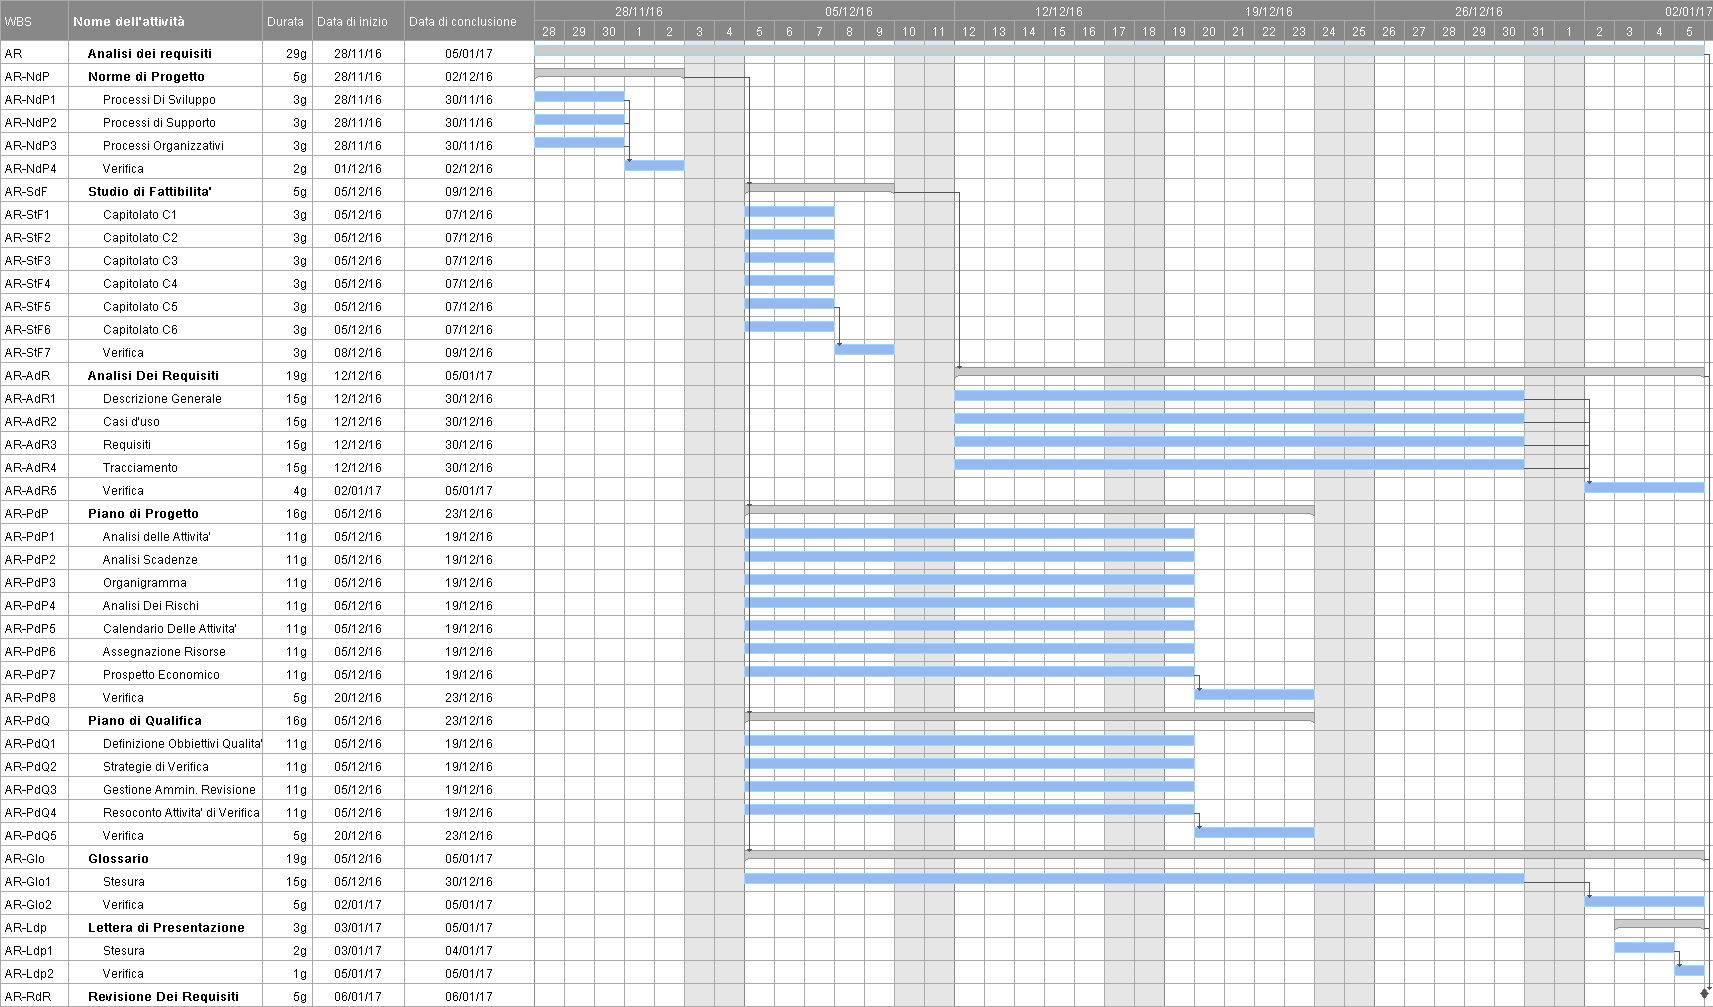
\includegraphics[angle=90,scale=0.37]{img/ganttnetbreak1.png}
			\caption{Diagramma di Gantt relativo al periodo di Analisi dei Requisiti}
		\end{figure}
		%qua finisce tabella con gantt
		
		\subsubsection{\ARD}
		\textbf{Periodo}: dal 2017-01-25 al 2017-02-24.\\
		L'inizio di tale periodo coincide con la consegna dei documenti per la \RR\ e ha la durata di circa un mese, antecedentemente rispetto al periodo preposto alla \PA. Durante questo periodo, il gruppo può analizzare la valutazione emersa dalla \RR\ ed effettuare le opportune correzioni. In questo periodo, inoltre, l'obiettivo è consolidare i requisiti individuati e procedere con la correzione di tutti i documenti inerenti alla consegna. La scadenza segnalata è una scadenza puramente interna al gruppo \textit{\gruppo}.
		
		\begin{figure}[H]
			\centering
			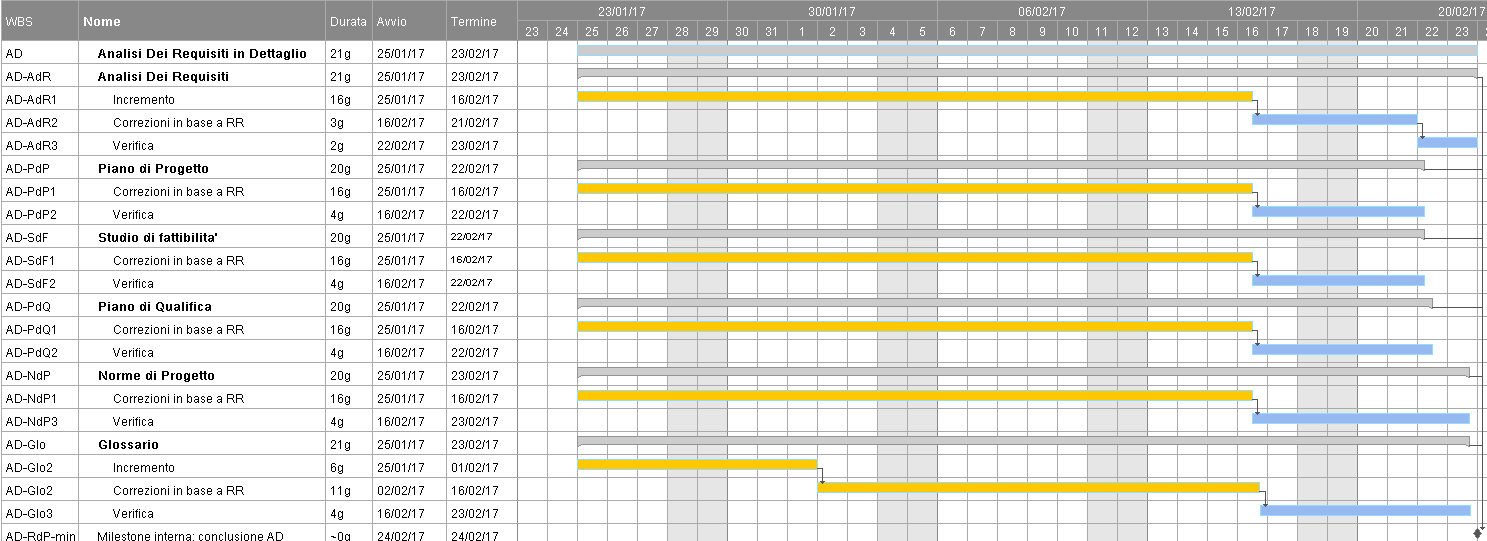
\includegraphics[scale=0.3]{img/ganttnetbreak2.png}
			\caption{Diagramma di Gantt relativo al periodo di Analisi dei Requisiti Dettagliata}
		\end{figure}
		
		
		\subsubsection{\PA}
		\textbf{Periodo}: dal 2017-02-25 al 2017-03-13.\\
		Il periodo di \PA\ inizia immediatamente dopo l'\AR\ e termina con la milestone prestabilita di \RPMin. Nell'arco di questo periodo è necessario effettuare la progettazione ad alto livello del sistema. Inoltre, si richiede di svolgere le seguenti attività:
		\begin{itemize}
			\item \textit{\ST}: documento che interessa prevalentemente il \textit{\Prog}\ del team. In esso vengono specificate:
			\begin{itemize}
				\item Scelte progettuali di alto livello prese;
				\item Design pattern scelti per la realizzazione del prodotto;
				\item Architettura generale del software.
			\end{itemize}
			\item Migliorare i documenti \NdP, \PdP, \PdQ\ e \G;
			\item Verificare e approvare tutti i documenti modificati.
		\end{itemize}
		I ruoli maggiormente interessati in questo periodo sono: \textit{\Amm}, \textit{\Res}, \textit{\Prog} e \textit{\Ver}.
		
		%qua inizia tabella con gantt
		%ho usato smartsheet, un'app web
		\begin{figure}[H]
			\centering
			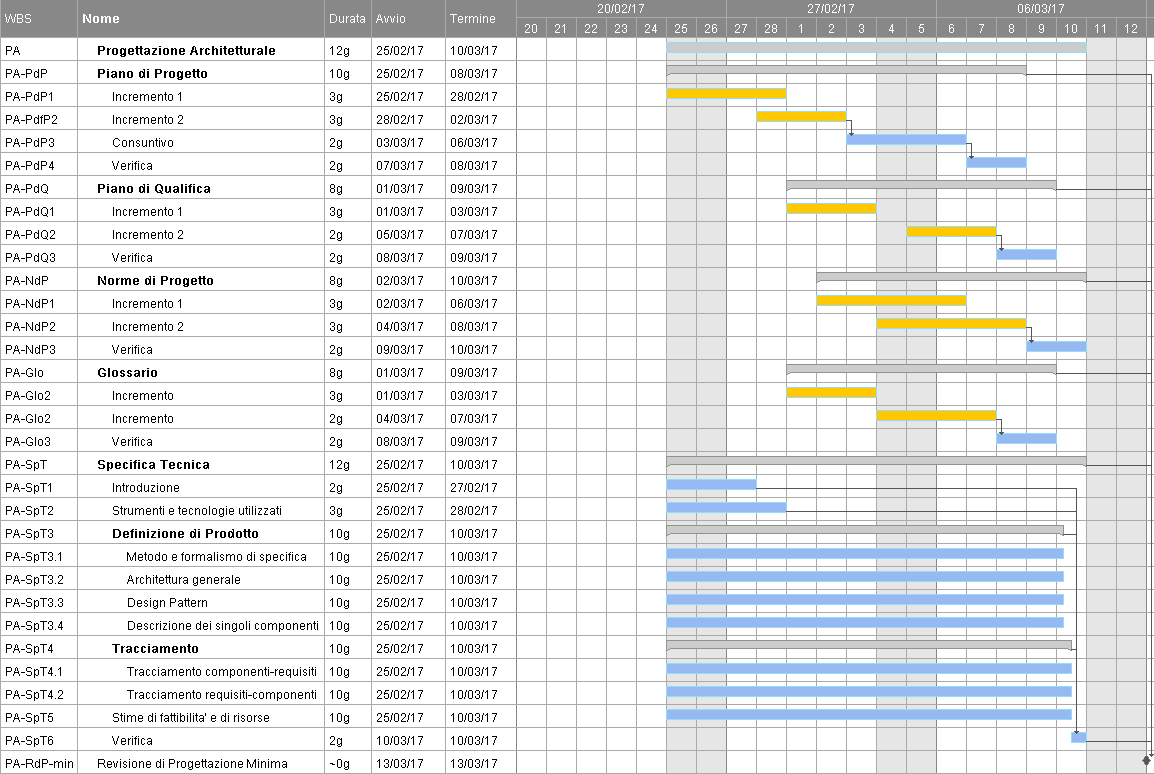
\includegraphics[scale=0.4]{img/ganttnetbreak3.png}
			\caption{Diagramma di Gantt relativo al periodo di Progettazione Architetturale}
		\end{figure}

		%qua finisce tabella con gantt
	
		\subsubsection{\PD}
		\textbf{Periodo}: dal 2017-03-14 al 2017-03-24.\\
		Il periodo di \PD\ inizia dopo quello di \PA\ e, in un'ottica di una progettazione di minimo, viene incorporata con la consegna dei documenti previsiti dalla \RQ. Questo periodo prevede la stesura dettagliata dell’intero sistema, specificando approfonditamente il comportamento e l’interazione tra i vari componenti. La scadenza individuata per questo periodo è puramente interna, dal momento che come è stato menzionato in precedenza, il gruppo NetBreak affronterà la progettazione con un livello di dettaglio intermedio (e non in una progettazione di massima per la scadenza della \RP).
		La Progettazione Architetturale Dettagliata prevede lo svolgimento delle seguenti attività:
		\begin{itemize}
			\item \textit{\DDP}: documento di responsabilità del \textit{\Prog}, il quale ha il compito di descrivere il comportamento	e le interazioni tra i vari componenti del sistema, basandosi sul documento di \ST;
			\item  Migliorare i documenti \NdP, \PdP, \PdQ, \ST\ e \G;
			\item Verificare e approvare tutti i documenti modificati.
		\end{itemize}
		I ruoli maggiormente interessati in questo periodo sono: \textit{\Amm}, \textit{\Res}, \textit{\Prog}\ e \textit{\Ver}.
		
		%qua inizia tabella con gantt
		%ho usato smartsheet, un'app web
		\begin{figure}[H]
			\centering
			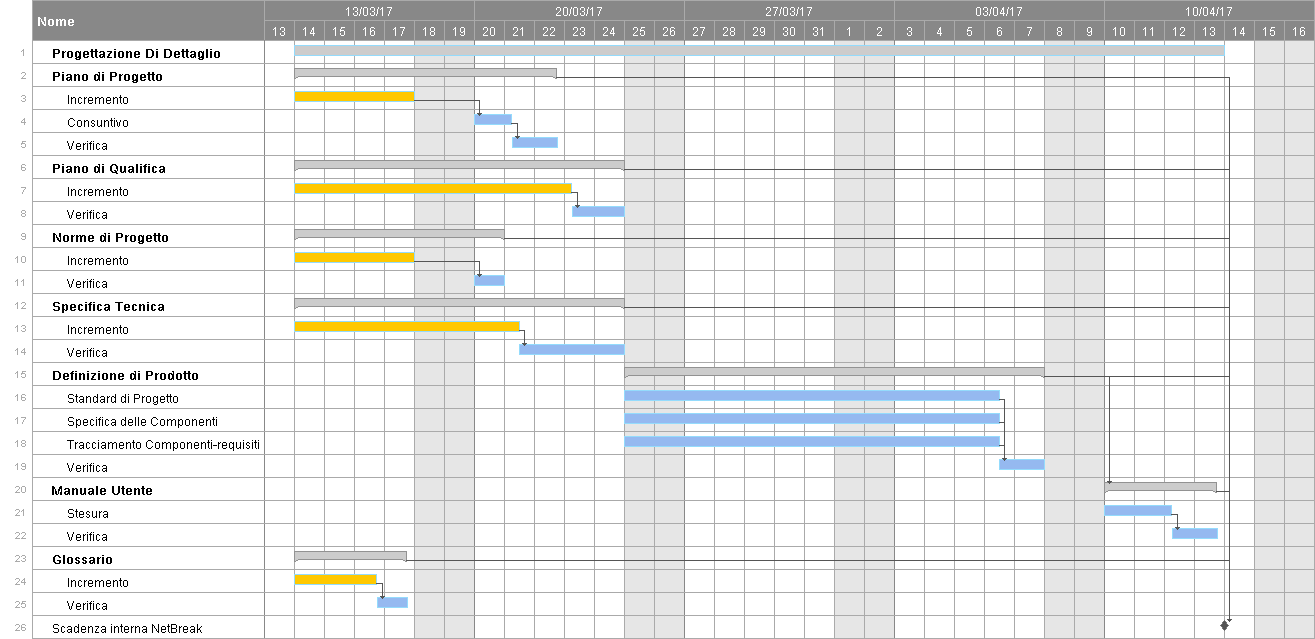
\includegraphics[scale=0.43]{img/ganttnetbreak4.png}
			\caption{Diagramma di Gantt relativo al periodo di Progettazione Architetturale Dettagliata}
		\end{figure}
		%qua finisce tabella con gantt
		
		\subsubsection{\CO}
		\textbf{Periodo}: dal 2017-03-25 al 2017-04-18.\\
		Il periodo di \CO\ è successivo alla \PD\ e si conclude con la consegna del prodotto per la \RQ. Questo periodo ha l'obiettivo di fornire un prodotto qualificato, grazie allo svolgimento delle seguenti attività:
		\begin{itemize}
			\item \textbf{Codifica}: i \textit{\Progrs}\ hanno il compito di sviluppare il codice del prodotto software progettato nelle precedenti attività e descritto nel documento \DDP. L’attività di Codifica prevede due cicli incrementali per: il miglioramento
			di parti del sistema già esistenti e funzionanti, e l’aggiunta di nuove funzionalità al sistema stesso.
			Ogni incremento prevede tre attività:
			\begin{itemize}
				\item Progettazione dell’incremento da parte dei \textit{\Progs};
				\item Codifica da parte dei \textit{\Progrs} dell’incremento progettato;
				\item Verifica dell’incremento effettuato.
			\end{itemize}
			\item \textit{\MU}: documento che descrive le linee guida per il corretto utilizzo del prodotto. Esso è destinato all’utilizzatore finale/cliente;
			\item  Migliorare i documenti \NdP, \PdP, \PdQ\ e \G;
			\item Verificare e approvare tutti i documenti modificati.
		\end{itemize}
		I ruoli maggiormente interessati in questo periodo sono: \textit{\Amm}, \textit{\Res}, \textit{\Prog}, \textit{\Progr}\ e \textit{\Ver}.
		
		%qua inizia tabella con gantt
		%ho usato smartsheet, un'app web
		\begin{figure}[H]
			\centering
			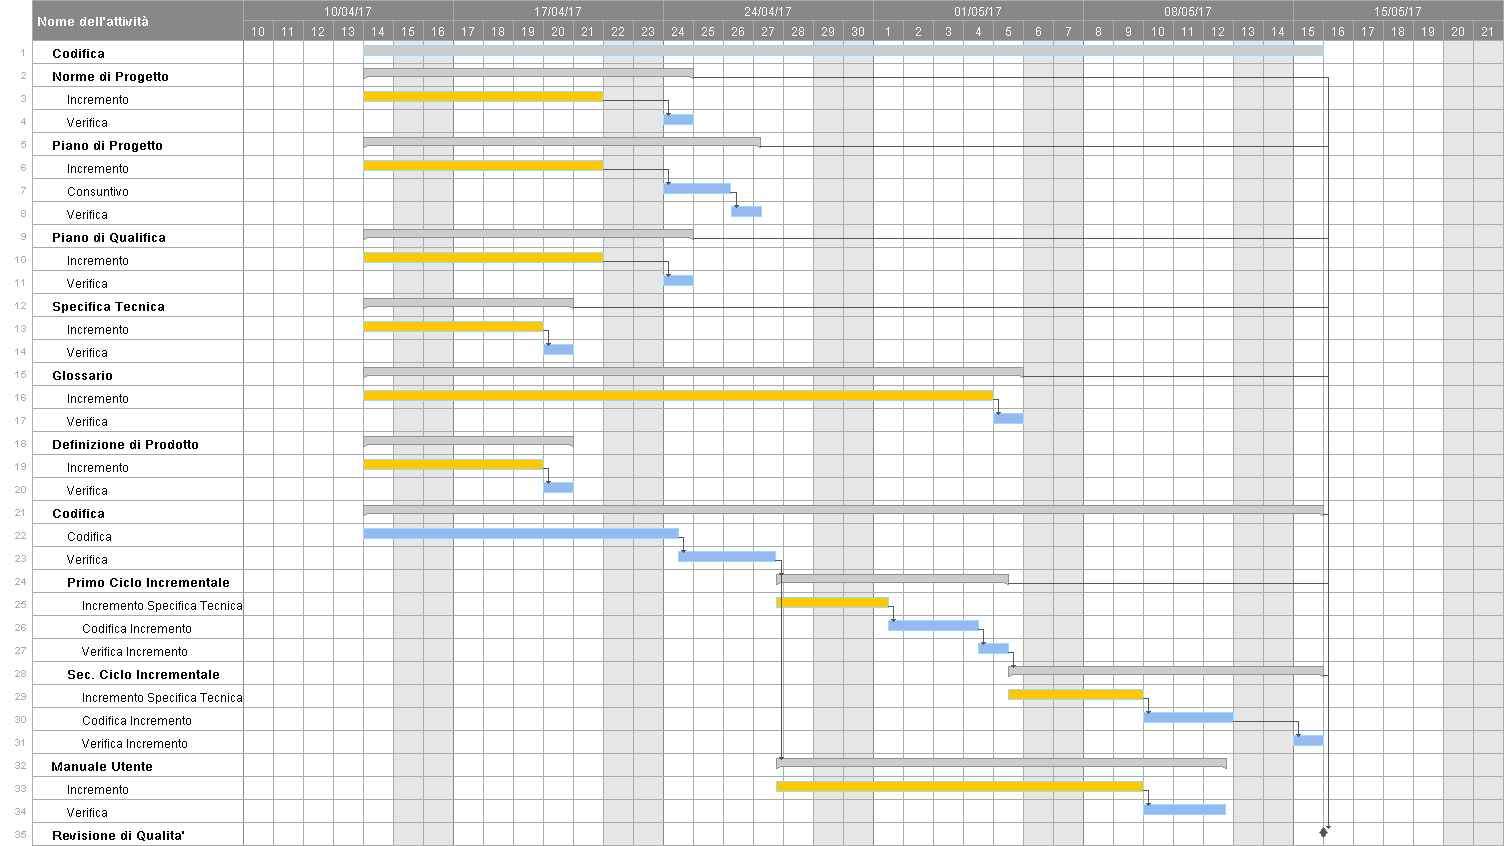
\includegraphics[scale=0.40]{img/ganttnetbreak5.png}
			\caption{Diagramma di Gantt relativo al periodo di Codifica}
		\end{figure}
		%qua finisce tabella con gantt
		
		\subsubsection{\VV}
		\textbf{Periodo}: dal 2017-04-19 al 2017-05-15.\\
		Il periodo di \VV\ inizia dopo quello di \CO\ e termina con la consegna del prodotto finale alla \RA. Questo periodo ha lo scopo di effettuare tutti i test necessari a garantire che il prodotto sia conforme alla attese e soddisfi tutti i requisiti concordati e descritti in \AdR. Le attività previste sono:
		\begin{itemize}
			\item Effettuare i test di sistema;
			\item Migliorare i documenti \NdP, \PdP, \PdQ, \G\ e \MU;
			\item Verificare e approvare tutti i documenti modificati.
		\end{itemize}
			I ruoli maggiormente interessati in questo periodo sono: \textit{\Res}, \textit{\Prog}\ e \textit{\Ver}.
			
		%qua inizia tabella con gantt
		%ho usato smartsheet, un'app web
		\begin{figure}[H]
			\centering
			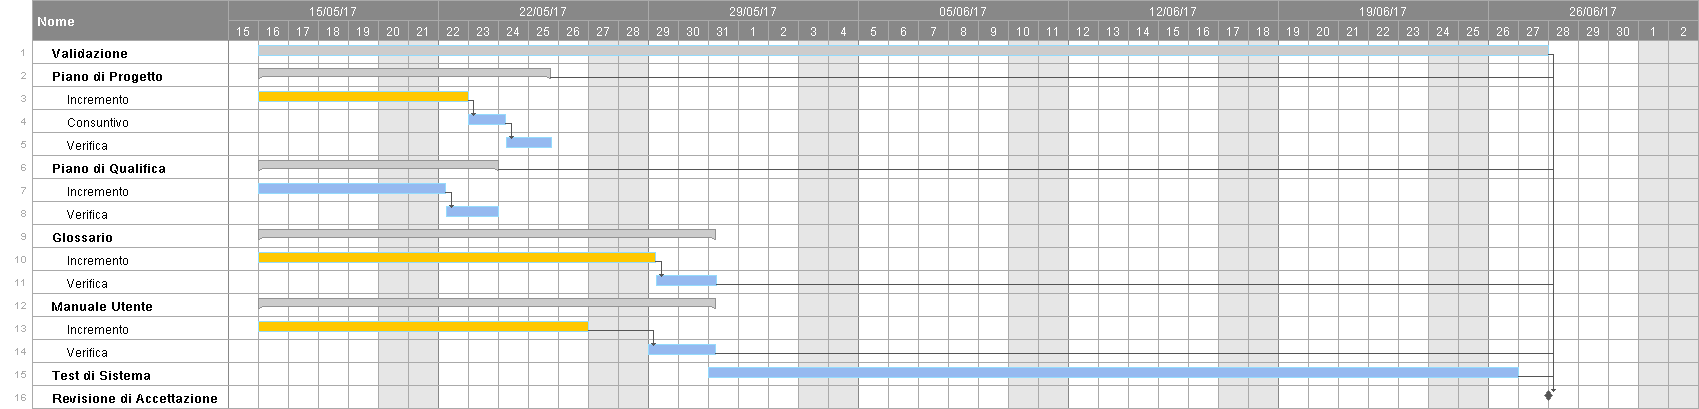
\includegraphics[scale=0.34]{img/ganttnetbreak6.png}
			\caption{Diagramma di Gantt relativo al periodo di Verifica e Validazione}
		\end{figure}
		%qua finisce tabella con gantt
\newpage
\section{Registro ore}
Nei seguenti paragrafi verrà spiegato come il gruppo intende dividere l'impegno dei ruoli nei sei diversi periodi di sviluppo del software. Successivamente verranno inserite le ore di investimento complessive nel gruppo. 
All'ultimo paragrafo, verrà mostrato un riassunto con il totale del peso dei vari ruoli nell'intero progetto.

\subsection{Periodo di Analisi dei Requisiti}
Il primo periodo è l'\AdR. Esso non è rendicontabile ai fini di calcolo del preventivo, poichè non è da considerarsi a carico del \textit{Proponente}. Le ore totali sono suddivise come segue:

\begin{table}[H]
	\begin{center}
		\begin{tabular}{|c|c|c|}
			\hline
			\textbf{Ruolo}	& \textbf{Ore}	& \textbf{Ore rendicontabili} \\
			\hline
			\Res	&	38	&  0 \\
			\hline
			\Amm	&	11	&  0 \\
			\hline
			\Ana	&	79	&  0 \\
			\hline
			\Ver	&	61	&  0 \\
			\hline
			\textbf{Totale} & \textbf{189} & \textbf{0} \\
			\hline
		\end{tabular}
	\end{center}
	\caption{Ore per ruolo, periodo di Analisi dei Requisiti}
\end{table}

L'incidenza di tali ore determina in percentuale, come mostrato di seguito:
\begin{figure}[H]
	\centering
	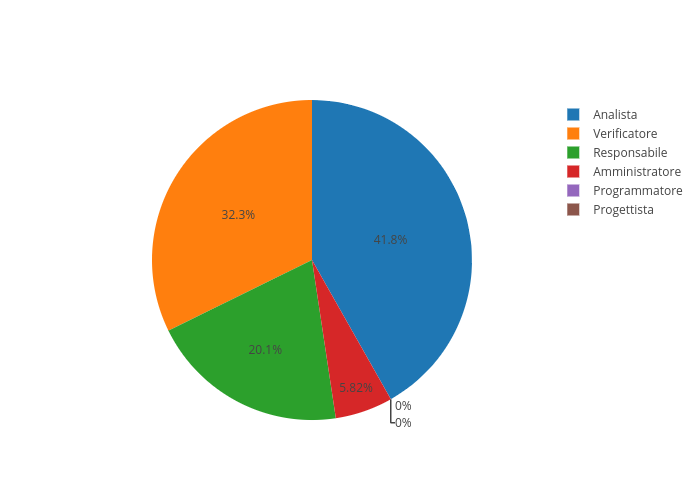
\includegraphics[scale=0.6]{img/AnalisiRequisiti.png}
	\caption{Incidenza ore per ruolo, periodo di Analisi dei Requisiti}
\end{figure}

\subsection{Periodo di Analisi dei Requisiti Dettagliata}
La seconda porzione di \AdR, da svolgersi dopo la \RR, è l'Analisi dei Requisiti Dettagliata. Come per il precedente, esso è da considerarsi parte dell'investimento intrapreso e quindi, non è rendicontabile ai fini del calcolo del preventivo. Le ore totali sono suddivise come segue:

\begin{table}[H]
	\begin{center}
		\begin{tabular}{|c|c|c|}
			\hline
			\textbf{Ruolo}	& \textbf{Ore}	& \textbf{Ore rendicontabili} \\
			\hline
			\Res	&   4 	&  0  \\
			\hline
			\Amm	&   1	&  0	\\
			\hline
			\Ana	&   5	&  0	\\
			\hline
			\Ver	&   5	&  0	\\
			\hline
			\textbf{Totale} & \textbf{15} & \textbf{0} \\
			\hline
		\end{tabular}
	\end{center}
	\caption{Ore per ruolo, periodo di Analisi dei Requisiti Dettagliata}
\end{table}

L'incidenza di tali ore determina in percentuale, come mostrato di seguito:
\begin{figure}[H]
	\centering
	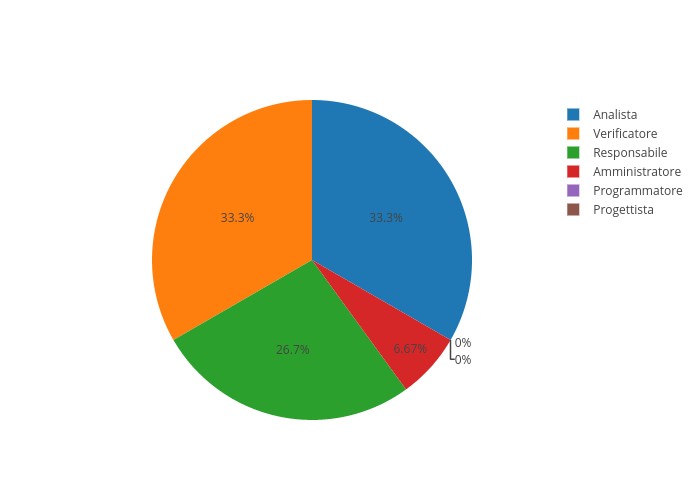
\includegraphics[scale=0.6]{img/AnalisiRequisitiDettaglio.png}
	\caption{Incidenza ore per ruolo, periodo di Analisi dei Requisiti Dettagliata}
\end{figure}

\subsection{Periodo di Progettazione Architetturale}
Lo sviluppo procede con la Progettazione Architetturale. Le ore totali sono suddivise come segue:

\begin{table}[H]
	\begin{center}
		\begin{tabular}{|c|c|c|}
			\hline
			\textbf{Ruolo}	& \textbf{Ore}	& \textbf{Ore rendicontabili} \\
			\hline
			\Res	&	5	&	5	\\
			\hline
			\Amm	&	5	&	5	\\
			\hline
			\Prog   &	138   &	138	\\
			\hline
			\Ver	&	52	&	52	\\
			\hline
			\textbf{Totale} & \textbf{200} & \textbf{200} \\
			\hline
		\end{tabular}
	\end{center}
	\caption{Ore per ruolo, periodo di Progettazione Architetturale}
\end{table}

L'incidenza di tali ore determina in percentuale, come mostrato di seguito:
\begin{figure}[H]
	\centering
	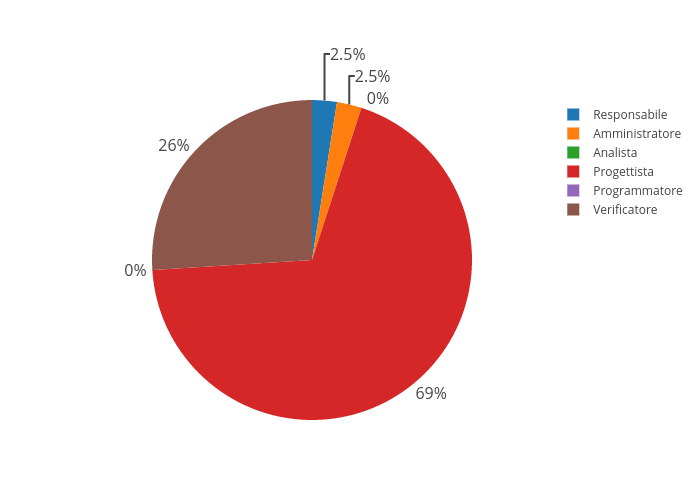
\includegraphics[scale=0.6]{img/ProgettazioneArchitetturale.png}
	\caption{Incidenza ore per ruolo, periodo di Progettazione Architetturale}
\end{figure}

\subsection{Periodo di Progettazione Architetturale Dettagliata}
Il terzo periodo è la Progettazione Architetturale Dettagliata. Le ore totali sono suddivise come segue:

\begin{table}[H]
	\begin{center}
		\begin{tabular}{|c|c|c|}
			\hline
			\textbf{Ruolo}	& \textbf{Ore}	& \textbf{Ore rendicontabili} \\
			\hline
			\Res	&	5	&	5 \\
			\hline
			\Amm	&	6	&	6	\\
			\hline
			\Prog   &	72   &	72	\\
			\hline
			\Ver	&	35	&	35	\\
			\hline
			\textbf{Totale} & \textbf{118} & \textbf{118} \\
			\hline
		\end{tabular}
	\end{center}
	\caption{Ore per ruolo, periodo di Progettazione Architetturale Dettagliata}
\end{table}

L'incidenza di tali ore determina in percentuale, come mostrato di seguito:
\begin{figure}[H]
	\centering
	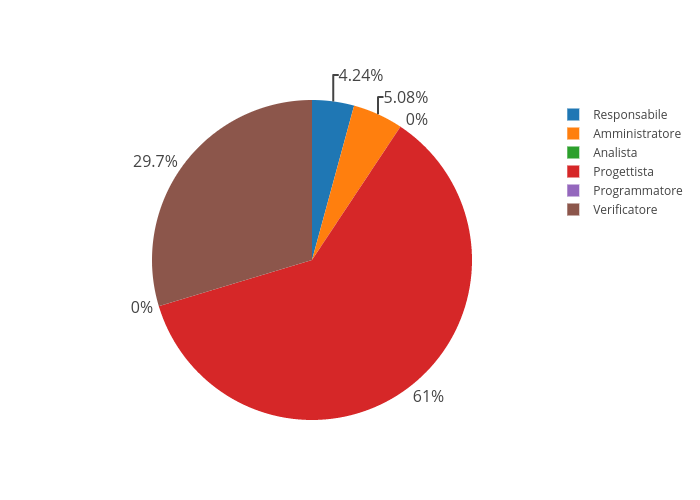
\includegraphics[scale=0.6]{img/ProgettazioneDettaglio.png}
	\caption{Incidenza ore per ruolo, periodo di Progettazione Architetturale Dettagliata}
\end{figure}

\subsection{Periodo di Codifica}
Il penultimo periodo è la Codifica. Le ore totali sono suddivise come segue:

\begin{table}[H]
	\begin{center}
		\begin{tabular}{|c|c|c|}
			\hline
			\textbf{Ruolo}	& \textbf{Ore}	& \textbf{Ore rendicontabili} \\
			\hline
			\Res	&	6	&	6	\\
			\hline
			\Amm	&	3	&	3	\\
			\hline
			\Progr   &	143   &	143	\\
			\hline
			\Ver	&	61	&	61	\\
			\hline
			\textbf{Totale} & \textbf{213} & \textbf{213} \\
			\hline
		\end{tabular}
	\end{center}
	\caption{Ore per ruolo, periodo di Codifica}
\end{table}

L'incidenza di tali ore determina in percentuale, come mostrato di seguito:
\begin{figure}[H]
	\centering
	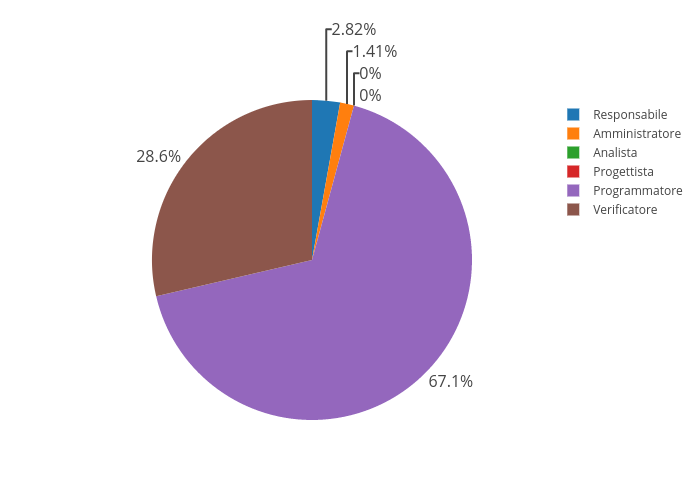
\includegraphics[scale=0.6]{img/Codifica.png}
	\caption{Incidenza ore per ruolo, periodo di Codifica}
\end{figure}

\subsection{Periodo di Verifica e Validazione}
L'ultimo periodo è la Verifica e Validazione del prodotto sviluppato. Le ore totali sono suddivise come segue:

\begin{table}[H]
	\begin{center}
		\begin{tabular}{|c|c|c|}
			\hline
			\textbf{Ruolo}	& \textbf{Ore}	& \textbf{Ore rendicontabili} \\
			\hline
			\Res	&	3  &	3	\\
			\hline
			\Amm	&	3  &	3	\\
			\hline
			\Prog   &	15  &	15	\\
			\hline
			\Ver	&	78	&	78	\\
			\hline
			\textbf{Totale} & \textbf{99} & \textbf{99} \\
			\hline
		\end{tabular}
	\end{center}
	\caption{Ore per ruolo, periodo di Verifica e Validazione}
\end{table}

L'incidenza di tali ore determina in percentuale, come mostrato di seguito:
\begin{figure}[H]
	\centering
	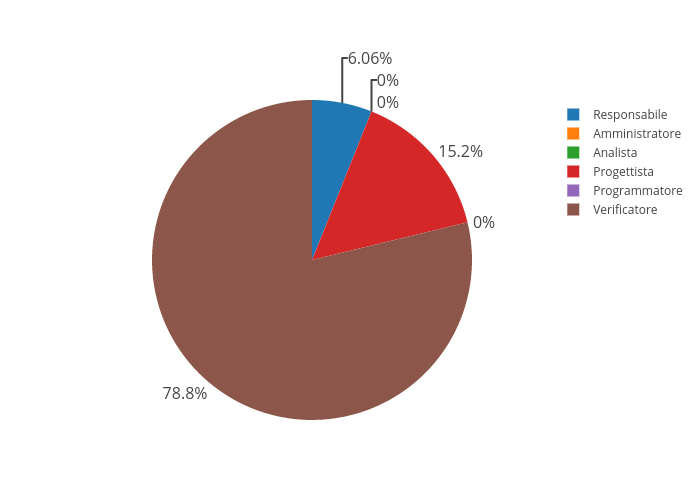
\includegraphics[scale=0.6]{img/Validazione.png}
	\caption{Suddivisione ore per ruolo, periodo di Verifica e Validazione}
\end{figure}

\subsection{Ore di investimento}
La quota di investimento comprende le ore necessarie ad apprendere le tecnologie richieste per la realizzazione del progetto. Queste ore esulano dalle ore di \textit{Analisi dei Requisiti} e non sono a carico del \textit{Proponente}. L'investimento delle ore per auto formazione sulle tecnologie necessarie allo svolgimento del progetto si è concentrato principalmente nel periodo di progettazione, come mostrato di seguito.
\begin{figure}[H]
	\centering
	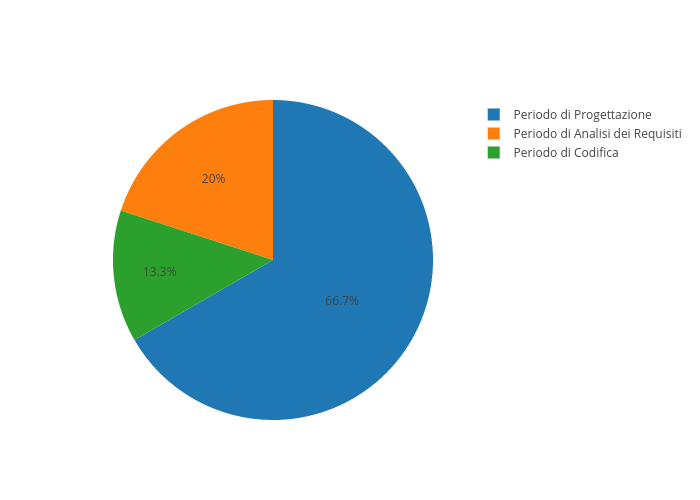
\includegraphics[scale=0.6]{img/ore_investimento_periodi}
	\caption{Ripartizione ore investimento}
	\label{fig:oreinvestimentoperiodi}
\end{figure}
Le ore complessive dedicate dai membri del gruppo sono 220 e riguardano auto formazione individuale sulle tecnologie necessarie e di indispensabile conoscenza da parte di tutti i membri del gruppo. Tutti i membri del gruppo, all'inizio del periodo di progettazione hanno affermato di avere buona padronanza delle seguenti tecnologie:
\begin{itemize}
	\item \textit{HTML5\ped{G}};
	\item \textit{CCS3\ped{G}};
	\item \textit{Java\ped{G}};
	\item \textit{MySQL\ped{G}}.
\end{itemize}
Le ore di auto formazione quindi, si sono concentrate sulle tecnologie rimanenti, ovvero:
\begin{itemize}
	\item \textit{Bootstrap 3\ped{G}};
	\item \textit{Jolie\ped{G}};
	\item \textit{JavaScript\ped{G}} e relativi framework:
	\begin{itemize}
		\item \textit{AngularJS\ped{G}};
		\item \textit{JQuery\ped{G}}.
	\end{itemize}
	\item \textit{Leonardo\ped{G}}.
\end{itemize}
Si segnala che un membro ha affermato di conoscere il framework \textit{Bootstrap 3}, per cui tralascerà l'auto formazione su tale tecnologia.

Di seguito sono riportate le ore che ogni membro ha dedicato all'auto formazione relativa alle tecnologie:

\begin{table}[H]
	\begin{center}
		\begin{tabular}{|c|c|}
			\hline
			\textbf{Ruolo}	& \textbf{Ore dedicate}  \\
			\hline
			\MC	&	33		\\
			\hline
			\DAN	&	34	\\
			\hline
			\AN	&	34		\\
			\hline
			\AS	&	31		\\
			\hline
			\NS	&	33		\\
			\hline
			\DS	&	32		\\
			\hline
			\textbf{Totale} & \textbf{197}  \\
			\hline
		\end{tabular}
	\end{center}
	\caption{Ore per auto formazione sulle tecnologie}
\end{table}


\subsection{Riepilogo}
Le ore totali del necessarie allo sviluppo sono 837 di cui, scorporando la fase di Analisi dei Requisiti, 630 remunerabili. Complessivamente le ore sono suddivise come segue:

\begin{table}[H]
	\begin{center}
		\begin{tabular}{|c|c|c|}
			\hline
			\textbf{Ruolo}	& \textbf{Ore complessive} & \textbf{Ore rendicontabili} \\
			\hline
			\Res	&	61	&	19	\\
			\hline
			\Amm	&	29	&	17	\\
			\hline
			\Ana	&	84	&	0	\\
			\hline
			\Prog	&	225	&	225	\\
			\hline
			\Progr	&	143	&	143	\\
			\hline
			\Ver	&	292	&	226	\\
			\hline
			\textbf{Totale} & \textbf{834} & \textbf{630} \\
			\hline
		\end{tabular}
	\end{center}
	\caption{Ore per ruolo, Riepilogo}
\end{table}

L'incidenza di tali ore incide in percentuale, come mostrato di seguito, prima complessive e poi remunerative:
\begin{figure}[H]
	\centering
	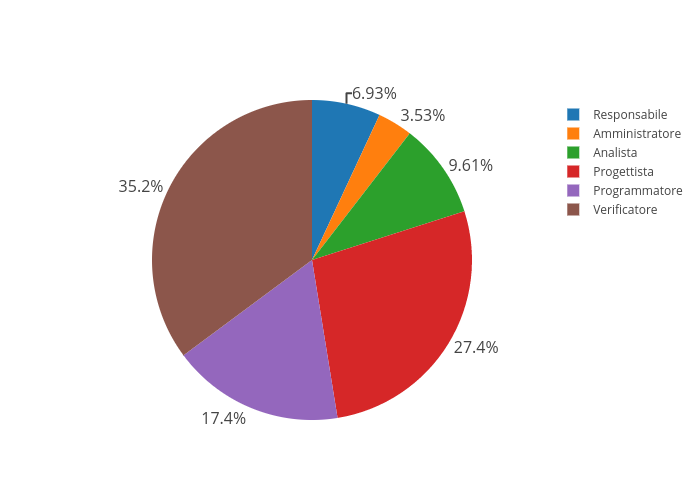
\includegraphics[scale=0.6]{img/OreTotali.png}
	\caption{Suddivisione ore per ruolo, riepilogo totale}
\end{figure}
\begin{figure}[H]
	\centering
	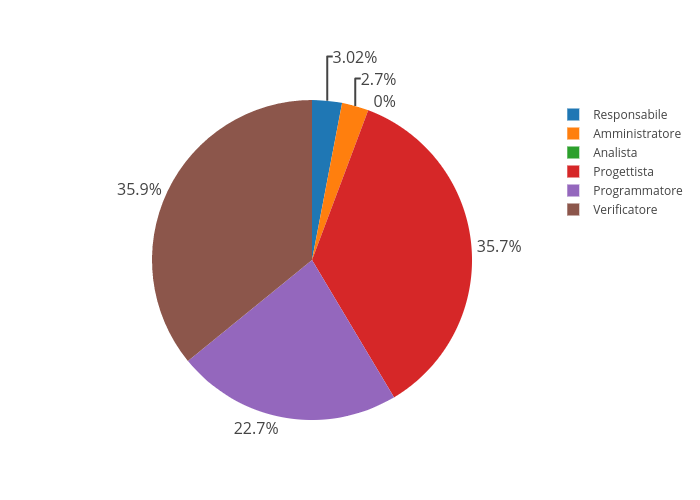
\includegraphics[scale=0.6]{img/OreRendicontabili.png}
	\caption{Suddivisione ore per ruolo, riepilogo ore remunerabili}
\end{figure}


\newpage

% template tabella!! Da cancellare solo quando finito
%\begin{table}[H]
%	\begin{center}
%		\begin{tabular}{|c|c|c|c|c|c|c|c|}
%			\hline
%			\textbf{nome} & \multicolumn{6}{c|}{\textbf{Ore per ruolo}} & \textbf{Ore totali} \\\cline{2-7}
%			& \textbf{Resp} & \textbf{Amm} & \textbf{An} & \textbf{Proj} & \textbf{Prog} & \textbf{Ver} & \\
%			\hline
%			\MC			&		&		&		&		&		&		&		\\
%			\hline
%			\AN			&		&		&		&	 	&		&		& 		\\
%			\hline
%			\DAN		&		&		&		&		&		&		&		\\
%			\hline
%			\AS			&		&	 	&	 	&		&	 	& 		&		\\
%			\hline
%			\NS 		&		&		&		&		&		& 		&		\\
%			\hline
%			\DS			& 		&		&		&		&		&		&		\\
%			\hline
%		\end{tabular}
%	\end{center}
%	\caption{Ore per componente, \AdR}
%\end{table}


\section{Registro suddivisione lavoro}
Nei seguenti paragrafi verrà spiegato come il gruppo intende dividere soddisfare alcune regole del progetto:
\begin{itemize}
	\item Tutti i componenti devono ricoprire almeno una volta tutti i ruoli; 
	\item Un componente del gruppo può ricoprire più ruoli contemporaneamente, a patto che non entri in conflitto d'interesse (ad esempio, non può verificare il lavoro da lui svolto).
\end{itemize}

\subsection{Periodo di Analisi dei Requisiti}
Durante il periodo di \AdR, il lavoro dei membri sarà suddiviso come segue:

\begin{table}[H]
	\begin{center}
		\begin{tabular}{|c|c|c|c|c|c|c|c|}
			\hline
			\textbf{Nome} & \multicolumn{6}{c|}{\textbf{Ore per ruolo}} & \textbf{Ore totali} \\\cline{2-7}
			& \textbf{Resp} & \textbf{Amm} & \textbf{An} & \textbf{Proj} & \textbf{Prog} & \textbf{Ver} & \\
			\hline
			\MC			&		&		&	16	&		&		&	16	&	32	\\
			\hline
			\AN			&		&	4	&	6	&	 	&		&	22	& 	32	\\
			\hline
			\DAN		&		&	3	&	29	&		&		&		&	32	\\
			\hline
			\AS			&	20	&	 	&	12 	&		&	 	& 		&	32	\\
			\hline
			\NS 		&	18	&	3	&	11	&		&		& 		&	32	\\
			\hline
			\DS			& 		&	2	&	5	&		&		&	25	&	32	\\
			\hline
		\end{tabular}
	\end{center}
	\caption{Ore per componente, \AdR}
\end{table}

\begin{figure}[H]
	\centering
	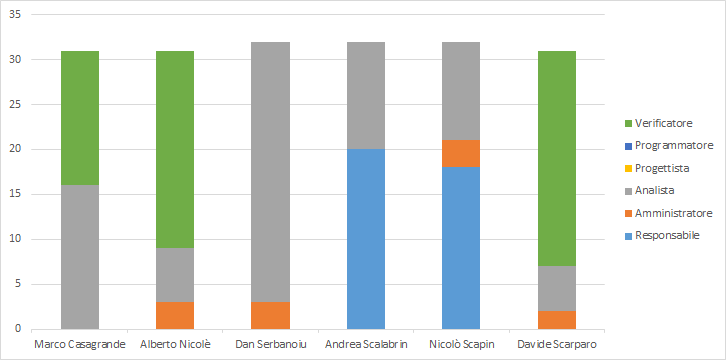
\includegraphics[scale=0.6]{img/6-1.png}
	\caption{Suddivisione ruoli per componente, Analisi dei Requisiti}
\end{figure}

\subsection{Periodo di Progettazione Architetturale}
Durante il periodo di Progettazione Architetturale, il lavoro dei membri sarà suddiviso come segue:

\begin{table}[H]
	\begin{center}
		\begin{tabular}{|c|c|c|c|c|c|c|c|}
			\hline
			\textbf{Nome} & \multicolumn{6}{c|}{\textbf{Ore per ruolo}} & \textbf{Ore totali} \\\cline{2-7}
			& \textbf{Resp} & \textbf{Amm} & \textbf{An} & \textbf{Proj} & \textbf{Prog} & \textbf{Ver} & \\
			\hline
			\MC			&		&	3	&		&	31	&		&		&   34	\\
			\hline
			\AN			&	3	&		&		&	31	&		&		& 	34	\\
			\hline
			\DAN		&		&	2	&		&	17	&		&	14	&	33	\\
			\hline
			\AS			&		&	 	&	 	&	14	&	 	& 	19	&	33	\\
			\hline
			\NS 		&		&		&		&	14	&		& 	19	&	33	\\
			\hline
			\DS			& 	2	&		&		&	31	&		&		&	33	\\
			\hline
		\end{tabular}
	\end{center}
	\caption{Ore per componente, Progettazione Architetturale}
\end{table}

\begin{figure}[H]
	\centering
	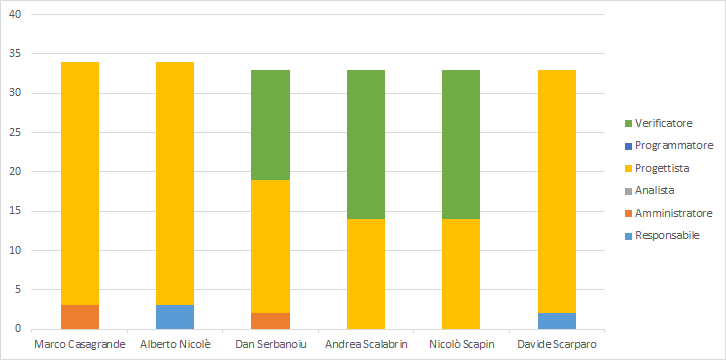
\includegraphics[scale=0.6]{img/6-2.png}
	\caption{Suddivisione ruoli per componente, Progettazione Architetturale}
\end{figure}

\subsection{Periodo di Progettazione Architetturale Dettagliata}
Durante il periodo di progettazione architetturale, il lavoro dei membri sarà suddiviso come segue:

\begin{table}[H]
	\begin{center}
		\begin{tabular}{|c|c|c|c|c|c|c|c|}
			\hline
			\textbf{Nome} & \multicolumn{6}{c|}{\textbf{Ore per ruolo}} & \textbf{Ore totali} \\\cline{2-7}
			& \textbf{Resp} & \textbf{Amm} & \textbf{An} & \textbf{Proj} & \textbf{Prog} & \textbf{Ver} & \\
			\hline
			\MC			&	2	&		&		&	6	&		&	11	&	19	\\
			\hline
			\AN			&		&		&		&	8	&   	&	11	& 	19	\\
			\hline
			\DAN		&	3	&		&		&	17	&		&		&	20	\\
			\hline
			\AS			&		&	3	&	 	&	17	&	 	& 		&	20	\\
			\hline
			\NS 		&		&	3	&		&	17	&		& 		&	20	\\
			\hline
			\DS			& 		&		&		&	7	&		&	13	&	20	\\
			\hline
		\end{tabular}
	\end{center}
	\caption{Ore per componente, Progettazione Architetturale Dettagliata}
\end{table}

\begin{figure}[H]
	\centering
	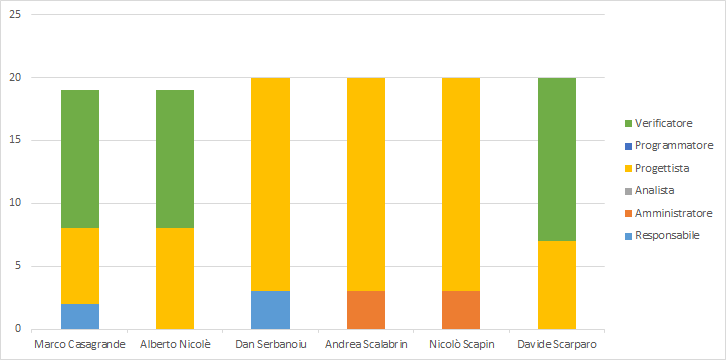
\includegraphics[scale=0.6]{img/6-3.png}
	\caption{Suddivisione ruoli per componente, Progettazione Architetturale Dettagliata}
\end{figure}

\subsection{Periodo di Codifica}
Durante il periodo di Codifica, il lavoro dei membri sarà suddiviso come segue:

\begin{table}[H]
	\begin{center}
		\begin{tabular}{|c|c|c|c|c|c|c|c|}
			\hline
			\textbf{Nome} & \multicolumn{6}{c|}{\textbf{Ore per ruolo}} & \textbf{Ore totali} \\\cline{2-7}
			& \textbf{Resp} & \textbf{Amm} & \textbf{An} & \textbf{Proj} & \textbf{Prog} & \textbf{Ver} & \\
			\hline
			\MC			&		&		&		&		&	18	&	18	&	36	\\
			\hline
			\AN			&	3	&		&		&	 	&	32	&		& 	35	\\
			\hline
			\DAN		&		&		&		&		&	14	&	21	&	35	\\
			\hline
			\AS			&		&	 	&	 	&		&	14 	& 	22	&	36	\\
			\hline
			\NS 		&		&	3	&		&		&	32	& 		&	35	\\
			\hline
			\DS			& 	3	&		&		&		&	33	&		&	36	\\
			\hline
		\end{tabular}
	\end{center}
	\caption{Ore per componente, Codifica}
\end{table}

\begin{figure}[H]
	\centering
	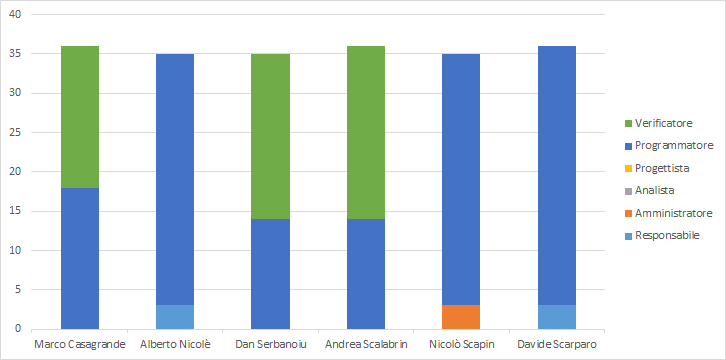
\includegraphics[scale=0.6]{img/6-4.png}
	\caption{Suddivisione ruoli per componente, Codifica}
\end{figure}

\subsection{Periodo di Verifica e Validazione}
Durante il periodo di Verifica e Validazione, il lavoro dei membri sarà suddiviso come segue:

\begin{table}[H]
	\begin{center}
		\begin{tabular}{|c|c|c|c|c|c|c|c|}
			\hline
			\textbf{Nome} & \multicolumn{6}{c|}{\textbf{Ore per ruolo}} & \textbf{Ore totali} \\\cline{2-7}
			& \textbf{Resp} & \textbf{Amm} & \textbf{An} & \textbf{Proj} & \textbf{Prog} & \textbf{Ver} & \\
			\hline
			\MC			&		&	3	&		&	7	&		&	6	&	16	\\
			\hline
			\AN			&		&		&		&	 	&		&	17	& 	17	\\
			\hline
			\DAN		&	3	&		&		&		&		&	14	&	17	\\
			\hline
			\AS			&		&	 	&	 	&	4	&	 	& 	12	&	16	\\
			\hline
			\NS 		&		&		&		&	4	&		& 	13	&	17	\\
			\hline
			\DS			& 		&		&		&		&		&	16	&	16	\\
			\hline
		\end{tabular}
	\end{center}
	\caption{Ore per componente, Verifica}
\end{table}

\begin{figure}[H]
	\centering
	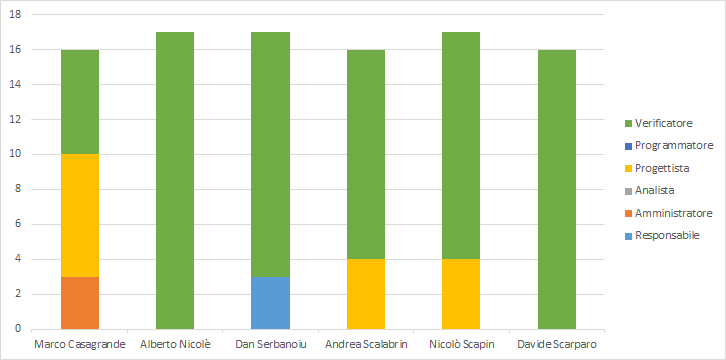
\includegraphics[scale=0.6]{img/6-5.png}
	\caption{Suddivisione ruoli per componente, Verifica}
\end{figure}

\subsection{Ore totali per componente}
Il consuntivo delle ore totali, raggruppate per ciascun membro del gruppo, e suddiviso per il ruolo assunto durante tutte le fasi del progetto, risulta essere così suddiviso:

\begin{table}[H]
	\begin{center}
		\begin{tabular}{|c|c|c|c|c|c|c|c|}
			\hline
			\textbf{Nome} & \multicolumn{6}{c|}{\textbf{Ore per ruolo}} & \textbf{Ore totali} \\\cline{2-7}
			& \textbf{Resp} & \textbf{Amm} & \textbf{An} & \textbf{Proj} & \textbf{Prog} & \textbf{Ver} & \\
			\hline
			\MC			&	2	&	6	&	16	&	44	&	18	&	51	&	137	\\
			\hline
			\AN			&	6	&	4	&	6	&	39	&	32	&	50	& 	137	\\
			\hline
			\DAN		&	6	&	5	&	29	&	34	&	14	&	49	&	137	\\
			\hline
			\AS			&	20	&	3 	&	12 	&	35	&	14 	& 	53	&	137	\\
			\hline
			\NS 		&	18	&	9	&	11	&	35	&	32	& 	32	&	137	\\
			\hline
			\DS			& 	5	&	2	&	5	&	38	&	33	&	54	&	137	\\
			\hline
		\end{tabular}
	\end{center}
	\caption{Ore totali, per componente}
\end{table}

\subsection{Ore totali remunerabili}
La tabella sottostante, infine, raccoglie il conteggio complessivo delle ore remunerabili, suddivise per ruolo e componente.

\begin{table}[H]
	\begin{center}
		\begin{tabular}{|c|c|c|c|c|c|c|c|}
			\hline
			\textbf{Nome} & \multicolumn{6}{c|}{\textbf{Ore per ruolo}} & \textbf{Ore totali} \\\cline{2-7}
			& \textbf{Resp} & \textbf{Amm} & \textbf{An} & \textbf{Proj} & \textbf{Prog} & \textbf{Ver} & \\
			\hline
			\MC			&	2	&	6	&	0	&	44	&	18	&	35	&	105	\\
			\hline
			\AN			&	6	&	0	&	0	&	39	&	32	&	28	& 	105	\\
			\hline
			\DAN		&	6	&	2	&	0	&	34	&	14	&	49	&	105	\\
			\hline
			\AS			&	0	&	3 	&	0 	&	35	&	14 	& 	53	&	105	\\
			\hline
			\NS 		&	0	&	6	&	0	&	35	&	32	& 	32	&	105	\\
			\hline
			\DS			& 	5	&	0	&	0	&	38	&	33	&	29	&	105	\\
			\hline
		\end{tabular}
	\end{center}
	\caption{Ore totali remunerabili, per ruolo e componente}
\end{table}

\newpage

\section{Quadro economico di progetto}
Si elenca, di seguito, il prospetto economico per il progetto: esso è suddiviso in sezioni riguardanti ciascuna fase dello stesso. Il piano economico così presentato, si basa sul calcolo delle ore presentato in precedenza. Sarà inserita, per scopo puramente conoscitivo, anche la fase di Analisi dei Requisiti, nonostante non sia rendicontabile e non rientri, quindi, nel calcolo complessivo. Di seguito, si illustrano i valori di riferimento per il calcolo dei costi:

\begin{table}[H]
	\begin{center}
		\begin{tabular}{|c|c|c|}
			\hline
			\textbf{Ruolo}	& \textbf{Costo per ora} \\
			\hline
			\Res	&	30	\\
			\hline
			\Amm	&	20	\\
			\hline
			\Ana	&	25	\\
			\hline
			\Prog	&	22	\\
			\hline
			\Progr	&	15	\\
			\hline
			\Ver	&	15	\\
			\hline
		\end{tabular}
	\end{center}
	\caption{Costo per ora, suddiviso per ruolo}
\end{table}

\subsection{Analisi dei Requisiti}
Il prospetto economico per quanto concerne l'Analisi dei Requisiti è il seguente:


\begin{table}[H]
	\begin{center}
		\begin{tabular}{|c|c|c|}
			\hline
			\textbf{Ruolo}	& \textbf{Numero di ore} & \textbf{Costo} \\
			\hline
			\Res	&	38  &	1140	\\
			\hline
			\Amm	&	12  &	240	\\
			\hline
			\Ana	&	79  &	1975	\\
			\hline
			\Ver	&	63  &	945	\\
			\hline
			\textbf{Totale}  &	192	&	4300	\\
			\hline
		\end{tabular}
	\end{center}
	\caption{Prospetto dei costi, Analisi dei Requisiti }
\end{table}

\begin{figure}[H]
	\centering
	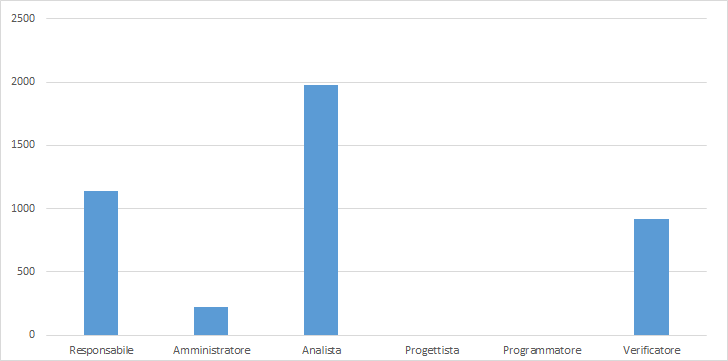
\includegraphics[scale=0.6]{img/8-1.png}
	\caption{Incidenza costi, Analisi dei Requisiti}
\end{figure}

\subsection{Progettazione Architetturale}
Il prospetto economico per quanto concerne la Progettazione Architetturale è il seguente:


\begin{table}[H]
	\begin{center}
		\begin{tabular}{|c|c|c|}
			\hline
			\textbf{Ruolo}	& \textbf{Numero di ore} & \textbf{Costo} \\
			\hline
			\Res	&	5  &	150	\\
			\hline
			\Amm	&	5  &	240	\\
			\hline
			\Prog	&	138  &	3036	\\
			\hline
			\Ver	&	52  &	780	\\
			\hline
			\textbf{Totale}  &	200 &	4206	\\
			\hline
		\end{tabular}
	\end{center}
	\caption{Prospetto dei costi, Progettazione Architetturale }
\end{table}

\begin{figure}[H]
	\centering
	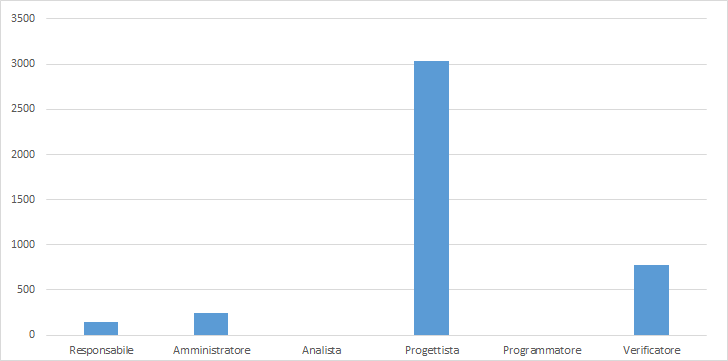
\includegraphics[scale=0.6]{img/8-2.png}
	\caption{Incidenza costi, Progettazione Architetturale}
\end{figure}

\subsection{Progettazione Architetturale Dettagliata}
Il prospetto economico per quanto concerne la Progettazione Architetturale Dettagliata è il seguente:


\begin{table}[H]
	\begin{center}
		\begin{tabular}{|c|c|c|}
			\hline
			\textbf{Ruolo}	& \textbf{Numero di ore} & \textbf{Costo} \\
			\hline
			\Res	&	5  &	150	\\
			\hline
			\Amm	&	6  &	120	\\
			\hline
			\Prog	&	72  &	1584	\\
			\hline
			\Ver	&	35  &	525	\\
			\hline
			\textbf{Totale}  &	118 &	2379	\\
			\hline
		\end{tabular}
	\end{center}
	\caption{Prospetto dei costi, Progettazione Architetturale Dettagliata }
\end{table}

\begin{figure}[H]
	\centering
	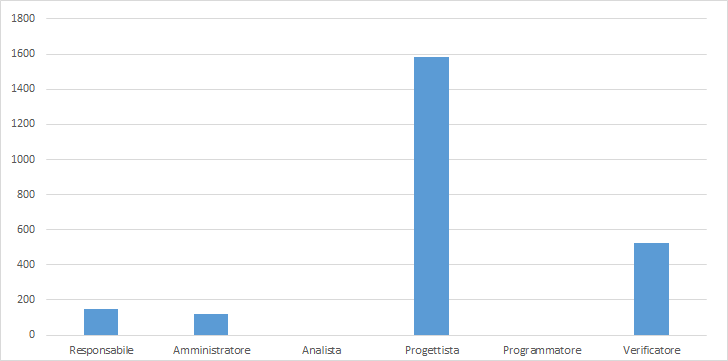
\includegraphics[scale=0.6]{img/8-3.png}
	\caption{Incidenza costi, Progettazione Architetturale Dettagliata}
\end{figure}

\subsection{Codifica}
Il prospetto economico per quanto concerne la Codifica è il seguente:


\begin{table}[H]
	\begin{center}
		\begin{tabular}{|c|c|c|}
			\hline
			\textbf{Ruolo}	& \textbf{Numero di ore} & \textbf{Costo} \\
			\hline
			\Res	&	6  &	180	\\
			\hline
			\Amm	&	3  &	60	\\
			\hline
			\Progr	&	143  &	2145	\\
			\hline
			\Ver	&	61  &	915	\\
			\hline
			\textbf{Totale}  &	213 &	3300	\\
			\hline
		\end{tabular}
	\end{center}
	\caption{Prospetto dei costi, Codifica }
\end{table}

\begin{figure}[H]
	\centering
	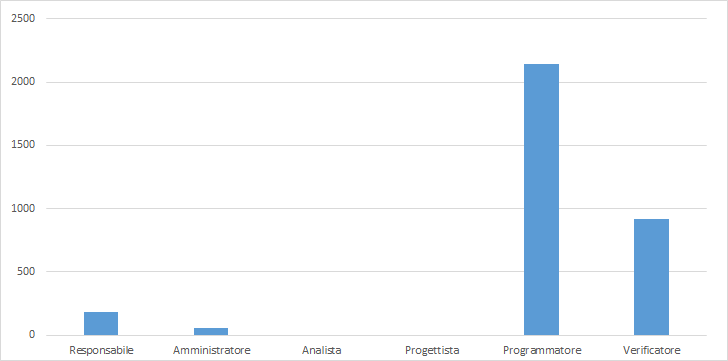
\includegraphics[scale=0.6]{img/8-4.png}
	\caption{Incidenza costi, Codifica}
\end{figure}

\subsection{Verifica e Validazione}
Il prospetto economico per quanto concerne la fase di verifica e validazione è il seguente:


\begin{table}[H]
	\begin{center}
		\begin{tabular}{|c|c|c|}
			\hline
			\textbf{Ruolo}	& \textbf{Numero di ore} & \textbf{Costo} \\
			\hline
			\Res	&	6  &	180	\\
			\hline
			\Prog	&	15  &	330	\\
			\hline
			\Ver	&	78  &	1170	\\
			\hline
			\textbf{Totale}  &	99  &	1680	\\
			\hline
		\end{tabular}
	\end{center}
	\caption{Prospetto dei costi, Verifica e Validazione}
\end{table}

\begin{figure}[H]
	\centering
	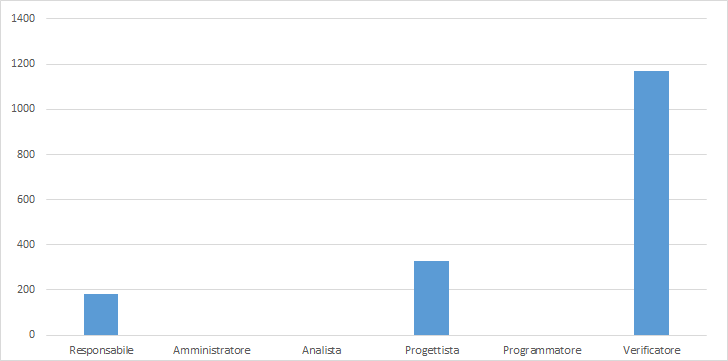
\includegraphics[scale=0.6]{img/8-5.png}
	\caption{Incidenza costi, Verifica}
\end{figure}

\subsection{Consuntivo totale e considerazioni conclusive}

Di seguito, la tabella mostra totale delle ore rendicontate, con il costo parziale e complessivo, suddiviso per ruolo. 

\begin{table}[H]
	\begin{center}
		\begin{tabular}{|c|c|c|}
			\hline
			\textbf{Ruolo}	& \textbf{Ore rendicontabili} & \textbf{Costo} \\
			\hline
			\Res	&	22  &	660	\\
			\hline
			\Amm	&	14  &	280	\\
			\hline
			\Prog	&	225  &	4950	\\
			\hline
			\Progr	&	143  &	2145	\\
			\hline
			\Ver	&	226  &	3390	\\
			\hline
			\textbf{Totale}  &	630  &	11425	\\
			\hline
		\end{tabular}
	\end{center}
	\caption{Prospetto dei costi complessivo}
\end{table}

\begin{figure}[H]
	\centering
	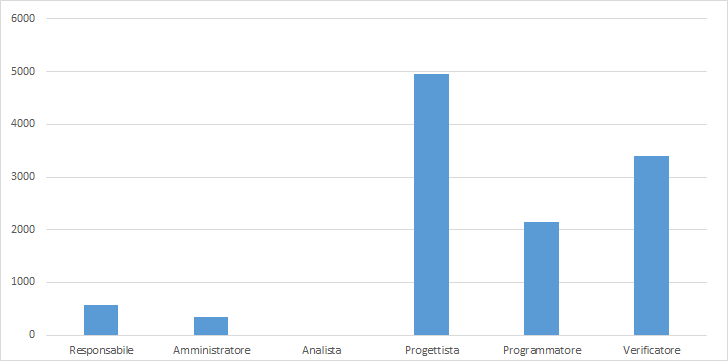
\includegraphics[scale=0.6]{img/8-6.png}
	\caption{Incidenza costi complessiva}
\end{figure}

Il costo complessivo preventivato per la realizzazione del progetto è, quindi, di \textbf{€ 11425}.
\newpage

\section{Consuntivi di periodo}

In questa porzione del documento verrà analizzato lo scostamento tra il preventivo calcolato e le ore effettive impiegate, sia in termini puramente di tempistiche, che di preventivo vero e proprio. Si potrà avere, dunque, uno scostamento in \textbf{Positivo}, qualora le ore impiegate siano minori delle ore preventivate, o in \textbf{Pari}, se il preventivo risulta corretto, oppure in \textbf{Negativo}, se la pianificazione per un determinato periodo è stata sottostimata.

\subsection{Analisi dei Requisiti}

Di seguito, si analizzano le ore realmente impiegate per ciascun componente, con l'eventuale scostamento in positivo o negativo indicato tra parentesi.

\begin{table}[H]
	\begin{center}
		\begin{tabular}{|c|c|c|c|c|c|c|c|}
			\hline
			\textbf{Nome} & \multicolumn{6}{c|}{\textbf{Ore per ruolo}} & \textbf{Totale} \\\cline{2-7}
			& \textbf{Resp} & \textbf{Amm} & \textbf{An} & \textbf{Proj} & \textbf{Prog} & \textbf{Ver} & \\
			\hline
			\MC			&		&		&	16	&		&		&	15 (-1)	&	31 (-1)	\\
			\hline
			\AN			&		&	3	&	6	&	 	&		&	22 (-2)	& 	31 (-2)	\\
			\hline
			\DAN		&		&	3	&	29 	&		&		&		&	32	\\
			\hline
			\AS			&	20	&	 	&	12 (+1) 	&		&	 	& 		&	32 (+1)	\\
			\hline
			\NS 		&	18 (-1)	&	3	&	11	&		&		& 		&	32 (-1)	\\
			\hline
			\DS			& 		&	2	&	5	&		&		&	24 (-2)	&	31 (-2)	\\
			\hline
			\textbf{Totali per ruolo}	& 	38 (-1)	&	11	&	79 (+1)	&		&		&	61 (-5)	&	189 (-5)	\\
			\hline
			\textbf{Scostamento preventivo}	& 	+30€	&		&	-25€	&		&		&	+75€	&	+80€	\\
			\hline
		\end{tabular}
	\end{center}
	\caption{Scostamento ore per componente, \AdR}
\end{table}

\subsubsection{Considerazioni}
Come si evince, l'impegno di alcune ore in meno rispetto a quanto preventivato, per quanto concerne specialmente l'attività di Verifica, ha prodotto uno scostamento in positivo del preventivo di € 80. Tale costo è ininfluente ai fini del preventivo a finire, in quando il costo dell'\textit{Analisi dei Requisiti}\ non è a carico del \textit{Proponente}.


\newpage
\subsection{Analisi dei Requisiti Dettagliata}

Di seguito, vengono analizzate le ore realmente impiegate per ciascun componente, in relazione al periodo di Analisi dei Requisiti Dettagliata.

\begin{table}[H]
	\begin{center}
		\begin{tabular}{|c|c|c|c|c|c|c|c|}
			\hline
			\textbf{Nome} & \multicolumn{6}{c|}{\textbf{Ore per ruolo}} & \textbf{Totale} \\\cline{2-7}
			& \textbf{Resp} & \textbf{Amm} & \textbf{An} & \textbf{Proj} & \textbf{Prog} & \textbf{Ver} & \\
			\hline
			\MC			&		&	1	&	 	&		&		&	2 	&	 3	\\
			\hline
			\AN			&		&		&	3 (-1) 	&	 	&		&	 	& 	 3 (-1)	\\
			\hline
			\DAN		&		&	 	&	2 	&		&		&		&	 2	\\
			\hline
			\AS			&	2	&	 	&	  	&		&	 	& 		&	 2	\\
			\hline
			\NS 		&	2	&		&	 	&		&		& 		&	 2	\\
			\hline
			\DS			& 		&	 	&	 	&		&		&	3 	&	 3	\\
			\hline
			\textbf{Totali per ruolo}	& 	4	&	1	&	5 (-1)	&		&		&	5	&	15 (-1)	\\
			\hline
			\textbf{Scostamento preventivo}	& 		&		&	+25€	&		&		&	&	+25€	\\
			\hline
		\end{tabular}
	\end{center}
	\caption{Scostamento ore per componente, \ARD}
\end{table}

\subsubsection{Considerazioni}
Il periodo dell'Analisi dei Requisiti Dettagliata ha prodotto un risparmio minimo sul costo preventivato. Il positivo di € 25 per questo periodo, è un risparmio del team, in quanto il costo non è a carico del \textit{Proponente}\ e quindi questo risparmio non va ad intaccare il preventivo a finire.

\newpage
\subsection{Progettazione Architetturale}

Di seguito, si analizzano le ore realmente impiegate per ciascun componente, in relazione al periodo di Progettazione Architetturale.

\begin{table}[H]
	\begin{center}
		\begin{tabular}{|c|c|c|c|c|c|c|c|}
			\hline
			\textbf{Nome} & \multicolumn{6}{c|}{\textbf{Ore per ruolo}} & \textbf{Totale} \\\cline{2-7}
			& \textbf{Resp} & \textbf{Amm} & \textbf{An} & \textbf{Proj} & \textbf{Prog} & \textbf{Ver} & \\
			\hline
			\MC			&		&	3 (-1)	&		&	31		&		&		&   33	(-1)\\
			\hline
			\AN			&3 (-1)	&			&		&	31		&		&		& 	34 (-1)	\\
			\hline
			\DAN		&		&	2		&		&	17		&		&	14	&	33	\\
			\hline
			\AS			&		&		 	&	 	&	13 (+1)	&	 	& 	19	&	32 (+1)	\\
			\hline
			\NS 		&		&			&		&	14 (+2)	&		& 	18 (-1)	&	32 (+1)	\\
			\hline
			\DS			& 	2	&			&		&	30 (-1)	&		&		&	32 (-1)	\\
			\hline
			\textbf{Totali per ruolo}	& 	5 (-1)	&	5 (-1)	&		&	137 (+2)	&		&	50 (-1)	&	197 (-1)	\\
			\hline
			\textbf{Scostamento preventivo}	& 	+30€	&	+20€	&		&	-50€	&		&	+15€	&	+15€	\\
			\hline
		\end{tabular}
	\end{center}
	\caption{Scostamento ore per componente, Progettazione Architetturale}
\end{table}

\subsubsection{Considerazioni}
L'attività di progettazione ha causato diversi problemi e quindi un numero maggiore di ore impiegate in Progettazione. A causa di alcune incomprensioni progettuali e necessità di approfondire alcune situazioni critiche con il Proponente, si è verifcato uno scostamento in negativo di € 50 nella progettazione, ma la gestione del gruppo e del progetto ha portato a una riduzione delle ore del Responsabile, dell'Amministratore e del Verificatore.

\newpage
\subsection{Progettazione Architetturale Dettagliata}

Di seguito, si analizzano le ore realmente impiegate per ciascun componente, in relazione al periodo di Progettazione Architetturale Dettagliata.

\begin{table}[H]
	\begin{center}
		\begin{tabular}{|c|c|c|c|c|c|c|c|}
			\hline
			\textbf{Nome} & \multicolumn{6}{c|}{\textbf{Ore per ruolo}} & \textbf{Totale} \\\cline{2-7}
			& \textbf{Resp} & \textbf{Amm} & \textbf{An} & \textbf{Proj} & \textbf{Prog} & \textbf{Ver} & \\
			\hline
			\MC			&	2	&		&		&	6	&		&	11	&	19	\\
			\hline
			\AN			&		&		&		&	8	&   	&	11	& 	19	\\
			\hline
			\DAN		&	3	&		&		&	17	&		&		&	20	\\
			\hline
			\AS			&		&	3	&	 	&	17	&	 	& 		&	20	\\
			\hline
			\NS 		&		&	3	&		&	17 (+1)	&		& 		&	20 (+1)	\\
			\hline
			\DS			& 		&		&		&	7 (+2)	&		&	13	&	20 (+2)	\\
			\hline
			\textbf{Totali per ruolo}	& 	5 	&	6 	&		&	72 (+3)	&		&	50 	&	131 (+3)	\\
			\hline
			\textbf{Scostamento preventivo}	& 		&		&		&	-75€	&		&		&	-75€	\\
			\hline
		\end{tabular}
	\end{center}
	\caption{Scostamento ore per componente, Progettazione Architetturale Dettagliata}
\end{table}


\subsubsection{Considerazioni}
L'attività di progettazione dettagliata ha visto diverse ulteriori lacune da colmare, anche in seguito alle segnalazioni emerse in sede di Revisione di Progettazione. Ciò ha richiesto di conseguenza un numero maggiore di ore impiegate in Progettazione, anche in questo caso. Si registra dunque in questa sede uno scostamento in negativo di € 75, mantenendo invariati gli altri ruoli

\newpage
\subsection{Codifica}

Di seguito, si analizzano le ore realmente impiegate per ciascun componente, per quanto concerne il periodo di Codifica.

\begin{table}[H]
	\begin{center}
		\begin{tabular}{|c|c|c|c|c|c|c|c|}
			\hline
			\textbf{Nome} & \multicolumn{6}{c|}{\textbf{Ore per ruolo}} & \textbf{Totale} \\\cline{2-7}
			& \textbf{Resp} & \textbf{Amm} & \textbf{An} & \textbf{Proj} & \textbf{Prog} & \textbf{Ver} & \\
			\hline
			\MC			&		&		&		&		&	18	&	18	&	36	\\
			\hline
			\AN			&	3	&		&		&	 	&	32	&		& 	35	\\
			\hline
			\DAN		&		&		&		&		&	14	&	21 (-1)	&	35 (-1)	\\
			\hline
			\AS			&		&	 	&	 	&		&	14 	& 	22 (-1)	&	36	(-1)\\
			\hline
			\NS 		&		&	3	&		&		&	32	& 		&	35	\\
			\hline
			\DS			& 	3	&		&		&		&	33	&		&	36	\\
			\hline
			\textbf{Totali per ruolo}	& 	6 	&	3 	&		&		&	143	&	50 (-2) 	&	202 (-2)	\\
			\hline
			\textbf{Scostamento preventivo}	& 		&		&		&		&		&	+30€	&	+30€	\\
			\hline
		\end{tabular}
	\end{center}
	\caption{Scostamento ore per componente, Periodo di Codifica}
\end{table}

\subsubsection{Considerazioni}
Durante l'attività di Codifica tutto si è svolto in maniera relativamente ordinaria, permettendoci di rilevare a seguito della consuntivazione un risparmio di 2 ore nell'attività di verifica del codice prodotto. 

\newpage
\subsection{Consuntivo parziale}

Analizzando i dati ottenuti, si ottiene un consuntivo parziale per il periodo rendicontato. Esso è consultabile nella tabella sottostante:

\begin{table}[H]
	\begin{center}
		\begin{tabular}{|c|c|c|}
			\hline
			\textbf{Periodo analizzato}	& \textbf{Scostamento ore}	& \textbf{Scostamento preventivo} \\
			\hline
			\AdR	&	-5	&	+ 80 €	\\
			\hline
			\ARD	&	-1	&	+ 25€	\\
			\hline
			\PA   &		-1  &	+ 15 €	\\
			\hline
			\PD   &	+3  &	- 75 €	\\
			\hline
			\CO   &		-2  &	+ 30 €	\\
			\hline
			\textbf{Totale} & \textbf{-6} & \textbf{+75 €} \\
			\hline
		\end{tabular}
	\end{center}
	\caption{Scostamento ore parziale}
\end{table}

Il conteggio finale, in data attuale, mostra come le previsioni, nonostante gli imprevisti nel periodo di Progettazione Architetturale e Progettazione Architetturale Dettagliata, risultano in linea con le aspettative. Il saldo parziale risulta, infatti, in attivo di € 75: questo dato, seppur di moderata entità, ha l'importanza di mostrare come le stime effettuate siano corrette (per il periodo rendicontato) ai fini del calcolo di un preventivo.

\paragraph{Preventivo a finire}
Il risparmio è minimo, ma un bilancio attivo in questa fase e nel prossimo periodo di Progettazione Architetturale Dettagliata, permetterà di poter investire la plusvalenza nell'aumento di ore di Codifica permettendo di migliorare la qualità del prodotto in ingresso alla \textit{Revisione di Accettazione.}
\newpage
\section{Organigramma}

\subsection{Componenti del gruppo}
\begin{table}[H]
	\begin{center}
		\setlength{\extrarowheight}{\jot}
		\begin{tabular}{|c|c|p{6cm}|p{4.3cm}|}
			\hline
			\textbf{Nominativo} & \textbf{Matricola}& \raggedright \textbf{Indirizzo di posta elettronica}										& \textbf{Ruoli} \\[1ex]
			\hline
			\MC					& 1049532			& \href{mailto:marco.casagrande.5@studenti.unipd.it}{marco.casagrande.5@studenti.unipd.it}& \Amm, \Ana, \Ver	\\[1ex]
			\hline
			\AN					& 1089847			& \href{mailto:alberto.nicole.2@studenti.unipd.it}{alberto.nicole.2@studenti.unipd.it} 	& \Ana, \Ver 	\\[1ex]
			\hline
			\DAN				& 1072680			& \href{mailto:dan.serbanoiu@studenti.unipd.it}{dan.serbanoiu@studenti.unipd.it} 			& \Amm, \Ana 	\\[1ex]
			\hline
			\AS 				& 1071936			& \href{mailto:andrea.scalabrin.2@studenti.unipd.it}{andrea.scalabrin.2@studenti.unipd.it}& \Res, \Ana	\\[1ex]
			\hline
			\NS					& 1051106			& \href{mailto:nicolo.scapin.1@studenti.unipd.it}{nicolo.scapin.1@studenti.unipd.it} 		& \Res, \Amm, \Ana	\\[1ex]
			\hline
			\DS					& 1049135			& \href{mailto:davide.scarparo@studenti.unipd.it}{davide.scarparo@studenti.unipd.it} 		& \Amm, \Ana, \Ver 	\\[1ex]
			\hline
		\end{tabular}
	\end{center}
	\caption{Componenti}
\end{table}

\subsection{Redazione}
\begin{table}[htbp]
	\begin{center}
		\setlength{\extrarowheight}{\jot}
		\begin{tabular}{|c|c|p{6cm}|p{4.3cm}|}
			\hline
			\textbf{Nominativo} & \textbf{Data di redazione} & \textbf{Firma} \\[1ex]
			\hline
			\AS					& 2016-12-05					 & \myincludegraphics{img/firme/AS.png} \\[1ex]
			\hline
		\end{tabular}
	\end{center}
	\caption{Redazione}
\end{table}

\newpage
\subsection{Approvazione}
\begin{table}[htbp]
	\begin{center}
		\setlength{\extrarowheight}{\jot}
		\renewcommand\arraystretch{0.8} 
		\begin{tabular}{|c|c|p{6cm}|p{4.3cm}|}
			\hline
			\textbf{Nominativo}    		& \textbf{Data di approvazione} & \textbf{Firma}  \\[1ex]
			\hline
			\AS							& 2017-01-09						& \myincludegraphics{img/firme/AS.png}			\\[1ex]
			\hline
			\TV							&								& \myincludegraphics{img/firme/blank.png}		\\[1ex]
			\hline
		\end{tabular}
	\end{center}
	\caption{Approvazione}
\end{table}

\newpage
\subsection{Accettazione dei componenti}
\begin{table}[htbp]
	\begin{center}
		\setlength{\extrarowheight}{\jot}
		\renewcommand\arraystretch{0.8} 
		\begin{tabular}{|c|c|p{6cm}|p{4.3cm}|}
			\hline
			\textbf{Nominativo} & \textbf{Data di accettazione} & \textbf{Firma} \\[1ex]
			\hline 
			\MC					&	2017-01-09					& \myincludegraphics{img/firme/MC.png}	 \\
			\hline
			\AN					&	2017-01-09					& \myincludegraphics{img/firme/AN.png}	 \\
			\hline
			\DAN				&	2017-01-09					& \myincludegraphics{img/firme/DAN.png} \\
			\hline
			\AS					&	2017-01-09					& \myincludegraphics{img/firme/AS.png}	 \\
			\hline
			\NS					&	2017-01-09					& \myincludegraphics{img/firme/NS.png}  \\
			\hline
			\DS					&	2017-01-09					& \myincludegraphics{img/firme/DS.png}	 \\
			\hline
		\end{tabular}
	\end{center}
	\caption{Accettazione dei componenti}
\end{table}





\end{document}